\documentclass[
a4paper, 12pt, % Papierformat, Schriftgröße
titlepage, 		 % extra Titelseite statt einfacher Überschrift
twoside,			 % beidseitiger Druck
headsepline,	 % Trennlinie für die Kopfzeile
BCOR5mm,			 % Binderand 5 mm
idxtotoc, bibtotoc]{scrreprt}	% Index (soweit vorhanden) und Literaturliste weggelassen: bibtotoc
				       % im Inhaltsverzeichnis aufführen
% Dokumentenklasse ist aus dem KOMA-Script-Paket die SCRReprt-Klasse.

\usepackage{wsi-ra}
% \usepackage{svg}

%%%%%%%%%%%%%%%%%%%%%%%%%%%%%%%%%
% Gestaltung der Titelseite     %
%%%%%%%%%%%%%%%%%%%%%%%%%%%%%%%%%

\titlehead{\vspace{.5cm}\centering
\textbf{\textsc{Eberhard-Karls-Universität Tübingen}}\\
Wilhelm-Schickard-Institut für Informatik\\Lehrstuhl Rechnerarchitektur}

\subject{\large Bachelor thesis}
% Studien-, Bachelor-, Diplom- oder Masterarbeit

% Der Titel
\title{\begin{tabular}{p{11cm}}\centering\Large
myttile
\end{tabular}}


% Der Name des Autors
\author{\large Philipp Noel von Bachmann}
\date{} % Hier kein Datum eintragen!

% Die Betreuer sowie das Abgabedatum etc.
\publishers{\normalsize\centering\begin{tabular}{p{3cm}p{8cm}}
\textbf{Betreuer:} 	& Prof.\,Dr.\,rer.\,nat.~Andreas Zell\\
			& Wilhelm-Schickard-Institut für Informatik\\
      & \\
			& Maximus Mutschler\\
			& Wilhelm-Schickard-Institut für Informatik\\
      & \\
\textbf{Begonnen am:}	& \\
 			& \\
\textbf{Beendet am:}	& \today
\end{tabular}}


%%%%%%%%%%%%%%%%%%%%%%%%%%%%%%%%%
% Eidesstattliche Erklärung     %
%%%%%%%%%%%%%%%%%%%%%%%%%%%%%%%%%

\uppertitleback{\ \\[4ex]\centering
\begin{tabular}{>{\normalsize}p{4.5cm}>{\normalsize}p{4cm}}
\large\textbf{Erklärung} & \\[4ex] \multicolumn{2}{p{8.5cm}}{\normalsize
Hiermit versichere ich, diese Arbeit selbstständig verfasst und nur die
angegebenen Quellen benutzt zu haben.}\\
\\[2ex]\multicolumn{2}{p{8.5cm}}{\normalsize Tübingen am \today}\\[6ex]
\begin{tabular}{p{4.2cm}}\cline{1-1}\\\end{tabular}&\\
Max Mustermann
\end{tabular}}
\lowertitleback{} % Hier nichts eintragen!


%%%%%%%%%%%%%%%%%%%%%%%%%%%%%%%%%
% Beginn des Dokumentes         %
%%%%%%%%%%%%%%%%%%%%%%%%%%%%%%%%%

\begin{document}


%%%%%%%%%%%%%%%%%%%%%%%%%%%%%%%%%
% Titelei                       %
%%%%%%%%%%%%%%%%%%%%%%%%%%%%%%%%%

\pagenumbering{roman}		% kleine lateinische Seitenzahlen
\maketitle

\begin{abstract}
% \textbf{Kurzfassung. }Dieses Dokument soll zeigen, wie mit \LaTeXe{} eine Abschlussarbeit entsprechend
der Richtlinien am Lehrstuhl Rechnerarchitektur erstellt werden kann. Es handelt
sich hierbei weder um eine Einführung in \LaTeX, noch in wissenschaftliche
Methode oder Schreibweise. Es werden einige Stilelemente und häufige
Schwierigkeiten exemplarisch herausgegriffen und vorgestellt. Ferner soll kurz
Aufbau und Benutzung dieser Vorlage beschrieben werden. Weiterführende Literatur
ist im Anhang aufgeführt. Zu den hier dargestellten \LaTeX-Paketen existieren
weiterhin eigene Dokumentationen, die nicht alle im Literaturverzeichnis
aufgeführt sind. Diese Vorlage basiert auf dem \KOMAScript-Paket
\cite{Neukam2003}, da hier die Dokumentenklasse Report (\verb!scrreprt!)
verwendet wird. Wichtig ist, dass die getätigten Einstellungen in diesem
Dokument nicht verändert werden, außer wenn statt in deutscher lieber in
englischer Sprache geschrieben wird. Dazu sind bereits einige Pakete vorgesehen,
die aber z.\,T. mit Kommentaren versehen und somit nicht aktiv sind. Die Datei
\verb!Vorlage.tex! dient als Hauptdokument. Der eigentliche Text sollte aber in
einer eigenen Datei pro Kapitel geschrieben werden, die dann lediglich in das
Hauptdokument eingebunden werden müssen. Dieses Vorgehen wird mit einem Kapitel
beispielhaft dargestellt. Ebenso können vorhandene Quelltexte direkt in das
Dokument integriert oder als Pseudocode aufgelistet werden. Auch wird
beispielhaft die Verwendung von Unterabbildungen, langen und normalen Tabellen
sowie mathematischen Formeln gezeigt. Abschließend wird kurz auf weiterführende
Literatur eingegangen. Ebenso beispielhaft werden im Abkürzungsverzeichnis
einige Einträge vorgenommen. Generell sollen nur verwendete Abkürzungen, die
nicht im Duden enthalten sind, in dieses Verzeichnis aufgenommen werden.
\end{abstract}

% \chapter*{Danksagung}
Ich danke allen, die an dieser Arbeit mitgewirkt haben. Eine Danksagung ist
grundsätzlich nicht nötig und darf durchaus entfallen. Falls gewünscht, ist die
Danksagung an dieser Stelle einzufügen.





\tableofcontents		% Inhaltsverzeichnis
\cleardoublepage		% Erzeugt neue Leerseite. Muss ggf. auskommentiert werden.
\pagenumbering{arabic}		% Ab hier mit arabischen Zahlen numerieren


%%%%%%%%%%%%%%%%%%%%%%%%%%%%%%%%%
% Beginn der eigentlichen Arbeit%
%%%%%%%%%%%%%%%%%%%%%%%%%%%%%%%%%

\chapter{Introduction}
\section{Optimization in Neural Networks}
Optimization is a core part of the current deep neural networks, as it is the
foundation of the learning process. However, optimization in the context of deep
learning differs from traditional optimization in several ways. This section
focuses on these differences and other current challenges of optimization in
deep neural networks. Most of the sections are inspired by
\cite{Goodfellow-et-al-2016}.

\subsection{Difference to traditional optimization}\label{sub:1}
In traditional optimization, we usually optimize on the data we want to perform
later directly. However in deep learning, we usually don't have access to the
test data. Consider autonomous driving. Here, the data the self-driving agent
has to act on will be generated while driving, with no chance of getting it in
advance. But we can capture data of other cars and optimize on them indirectly.
The hope beeing, that the distribution of the training set is similar to the one
of the later test set, so that reducing training error will result in reducing
test error.

Formally, we want to reduce the test error given by
\begin{align}\label{eq:1}
    J(\theta) = E_{(x,y)\sim p_{data}} L(f(x;\theta), y)
\end{align}
where $L$ is the Loss-Function, $f(x;\theta)$ the output of the network with
respect to the input $x$ and parameters $\theta$, and $y$ the labels for the
input. This equation is known as \textbf{risk}. However, during the training
process, we only have access to the training set which is distibuted according 
to $\hat{p}_{data}$ rather than $p_{data}$. Therefore, we can only optimize
\begin{align}
    J(\theta) = E_{(x,y)\sim \hat{p}_{data}} L(f(x;\theta), y)
\end{align}
To overcome this issue, we use a technique called empirical risk minimization.

\subsection{Empirical risk minimization}\label{sub:2} As we have already seen,
although we cannot reduce the generalization risk of equation \ref{eq:1}, as we
only have the training data. To convert the problem back to a normal
optimization problem, we use the expectation over the empirical distribution.
This is known as \textbf{empirical risk minimization}. The arimethic mean
serves as an unbiased estimator for the true mean of $\hat{p}_{data}$.
\begin{align}\label{eq:3}
    J(\theta) = E_{(x,y)\sim \hat{p}_{data}} L(f(x;\theta), y) = \frac{1}{m} \sum_{i=1}^m L(f(x^{(i)}; \theta), y^{(i)})
\end{align}
As the training set from the empirical distribution is restricted in size, this
quickly leads to overfitting, where the network memorizes the training set.
Therefore, additional measurements like Regularization have to be taken into
account.


\subsection{Minibatch Algorithms}\label{sub:Minibatch}
We have seen in equation \ref{eq:3} that we use the mean over the whole training
set to approximate the empirical risk. From a computational perspective, this is
rather expensive. That's why we normally only use a subset of the training set
for each parameter update. These subsets are called \textbf{batches}. Some statistical
considerations justify this.

The standard error of mean is given by $\frac{\sigma}{n}$, where $n$ is the
number of training examples. The root in the denominator results in that, when
increasing the number of training examples, the standard error of mean will
only decrease sublinear. That's why it is unattractable to use large batches of
training data. The second factor is redundancy in the training set. As some
examples might be quite similar to each other, the mean of a subset will not
differ much from the whole training data, but requires much less computation
time.

Most loss-functions allow us to divide the data into batches easily. The most
common example for classification is maximum likelyhood, which is defined as:

\begin{align}
    \theta_{ML}
    & = argmax_{\theta} p_{model}(X; \theta) \\
    & = argmax_{\theta} \prod_{i=1}^m p_{model}(x^{(i)}; \theta)
\end{align}

If we convert it to log-space, the product decomposes into a sum:

\begin{align}
    \theta_{ML} = argmax_{\theta} \sum_{i=1}^m log p_{model}(x^{(i)}; \theta)
\end{align}

In this space, we can easily divide the sum into batches and train on them
seperatly. The same idea can be applied to the gradient:
\begin{align}
    \nabla_\theta J(\theta)=E_{x,y\sim \hat{p}_{data}} \nabla_\theta log(p_{model}(x,y;\theta))
\end{align}

Optimization algorithms which use the whole trainig set are called
\textbf{batch} or \textbf{deterministic} algorithms, while deterministic is
prefered, as the term batch is also used in minibatch methods. The other extreme
are \textbf{stochastic} or \textbf{online} methods, where only one training
example is processed at a time. In between lie the methods, where more than one
training example is used, but not all. These are called \textbf{minibatch}
methods and are most commonly used in machine learning. A typical example for
stochastic methods is stochastic gradient descent, see section \ref{SGD}.


Both methods have their advantages beyond the computational perspective. While
large batches offer a more accurate estimate of the gradient, small batches can
add a regularization effect. They add some noise to the gradient, and therefore
lead the optimization algorithm to areas, where a small inaccuracy in the
gradient converges to the same point. As the point is a very stable or wide
minimum, this results in a regularization effect which decreases the
generalization error. This is also supported by the work of Keskar et al.
\cite{keskar2016large}, who argued that larger batches converge to sharp
minimas, whereas small converge to flat. Section \ref{sub:Generalization} shows,
that flat minima are believed to be better in generalization. Therefore, a small
batch which ends up in a flat minima results in better generalization
capabilities.


The effect of batch size is also sensitive to the choice of the optimization
algorithm. In particular, second-order algorithms suffer from a small batch
size. Hessian matrices $H$ require a much larger sample size to be accurate than
the Jacobian. Especially when $H$ is of large condition number, this leads to the
an amplification of the preexisting errors in $g$.

To get an unbiased esimate of the gradient, it is important to sample the
mini-batches randomly. This is a problem in particular when the training data is
corellated. For example autocorellation can arise, when data is taken from a
time series. The problem can be overcome by sampling the minibatches uniformly
out of the training data. However, that would lead to a large computational
effort every time we want to construct a batch. Fortunally, it seems sufficient
to shuffle and divide the training data into batches only once.

Another property is that the gradient of minibatch algorithms like stochastic
gradient descent follow the true gradient, as long as the training data is only
used once. As each datapoint from the training set is only used once, it also
follows the true data distribution $p_{data}$. Therefore we get an estimate of
the true gradient. When reusing the data from $\hat{p}_{data}$, it no longer
follows $p_{data}$, so the estimation becomes inaccurate.

\subsection{Challenges in Neural Networks}
In the last part, we demonstrated how optimization in deep learning differs from
traditional optimization from a statistical point of view. This difference is
emphasized further by other factors, in particular the non-convex loss
landscape. This part will summarize some of these problems and their
implications for deep learning.


\subsubsection{Local Minima}\label{sub:Local_minima}
In convex optimization problems, every local minima is guaranteed to be the
global minima. Therefore finding a minimum is a sufficient enough condition to
stop. In neural networks however, the loss landscape is highly non-convex. This
results in a local minima possibly having higher cost value than the global
minima. Proofs that these local minima exist can be constructed quite easily.

One example is the weight space symetrie. Suppose you swap out nodes i and j by
swapping their incoming and outgoing weights. Then the activation in the next
and all subsequent layers of the networks will stay the same, but the networks
are located at different places in the loss landscape, therefore creating two
local minimas. Although a large number of these local minima exist, they form no
problem for optimization. As mentioned, the swap will lead to the same
activation, therefore the networks will performe the same on the data and the
value of these local minimas will be equal.

However, there can also exist local minima with high cost compared to the global
minimum. In theorie this was believed to be an issue, but in practice it seemed
to cause no problem. Recently, some theoretical work support these findings.
Chromanska et al. \cite{choromanska2015loss} applied spin glass theory from
physics to neural networks. This allowed them to verify that for large networks,
local extrema with higher cost are exponentially likely to be saddle points.
Therefore, all local minima are approximately of the same cost, which is close
to the global optimum and it is very unlikely to get stuck in a local minimum
with high cost.

\subsubsection{Saddle Points}\label{prob:3}
Saddle points are another type of local extrema where the gradient is 0. In
contrast to local maxima or minima where the Hessian only has negative or
positive eigenvalues, the Hessian of saddle points has both positive and
negative eigenvalues.

In fact, saddle points get more common for higher dimensional space. The idea of
coin flipping can be used to describe this phenomena. Suppose every eigenvalue
of the Hessian is generated by flipping a coin. In a low-dimensional space, it
quite likely that all of these flips will be positive or negative, resulting in
minima or maxima. The higher the dimension gets however, the more likely the
Hessian is to have both positive and negative eigenvalues. Therefore, there
exist more saddle points. Chromanska et al. \cite{choromanska2015loss} also
showed that these saddle points are more likely to occur in areas of higher
loss.

What problems arise from saddle points depends in the choice of the optimization
algorithm. For first-order algorithms, the situation is unclear. Although the
gradient might get small in regions close to saddle points and as a result could
slow down training, in pratice it seems like it isn't a problem for gradient
descent. Especially when adding Momentum to the algorithm, it is very unlikely
that that the gradient becomes 0, because there is no gradient in opposing
direction which would decrease the Momentum. For second-order algorithms, saddle
points are clearly a problem. Newton's algorithm for example explicitly solves
for point with zero gradient, and is therefore attracted to saddle points or
even other extrema like maxima. This is partly resolved by the introduction of
saddle-free Newton. 


\subsubsection{Vanishing gradients}\label{sub:Vanishing_gradient} Today's neural
network become very deep. But with increasing depth, there arises a problem
called vanishing and exploding gradient. It refers to the fact that when
back-propagating the gradient, it either vanishes or explodes. More formally,
consider a matrix $W$ which is multiplied by repeatedly on a computation path.
If a eigendecomposition $Vdiag(\lambda )V^{-1}$ exists, this results in
$(Vdiag(\lambda )V^{-1})^t=Vdiag(\lambda )^tV^{-1}$. Therefore, all values are
scaled according to the eigenvalues of $W$. If these eigenvalues are between 0
and 1, the gradient will vanish. If they are larger then 1, it will explode.
This especially occurs when the network becomes increasingly deep, as the power
of these eigenvalues is taken. One solution for this problem is the ResNet
architecture, which will be described in detail in section \ref{sub:ResNet}

\subsubsection{Poor correspondence between local and global
structure}\label{prob:5}

The previous sections have focused on which problems we are facing when
computing a gradient or updating locally. However, the local structure can often
be misleading. Local gradients can often point away from  or costruct a
subotimal path to areas of low loss. Even if we are able to perform the best
move locally and end up in a local minima, we are not guaranteed to be in the
globally best area. 

Figure \ref{fig:Poor_correspondence}
shows an example of suboptimal initialization. As the local structure for $x<0$
doesn't reflect the global, these initializations will not lead to the global
minimum. Therefore, theretical work has gone into finding good initialization
strategies.

\begin{figure}[h]\label{fig:Poor_correspondence}
    \begin{center}
        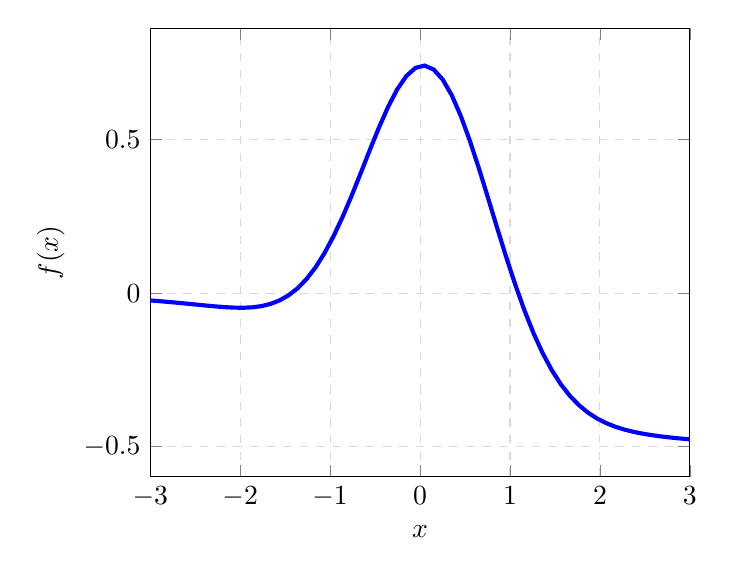
\begin{tikzpicture}
            \begin{axis}[
            grid=major, 
            grid style={dashed,gray!30},
            xlabel=$x$, % Set the labels
            ylabel=$f(x)$,
            xmin=-3,
            xmax=3]
            \addplot[mark=none,color=blue, line width=1.5pt, samples=100] {exp(-(x-0.1)^2)-0.5/(1+exp(-x))};%{exp(-x^2)-0.5*exp(-(x-2)^2)+1};
            \end{axis}
        \end{tikzpicture}
        \caption{Example of poor correspondence between local and global
        structure. If $x<0$ is initialized, gradient descent will lead us in
        negative direction. However, this leads away from the global optimum
        on the right.}
    \end{center}
\end{figure}

Another issue may be that there even is no global minimum. This happens for
example with the usage of the softmax, where the weights are increased without
bound even when the accuracy is very good. This occurs because the actual labels
for the softmax can only approach 1 with larger values, but never actually reach
it.  On solution to the second phenomena would be label smoothing, where instead
of a hard 0-1 coding of the classification, each of the 0 are replaced by
$\frac{k}{\textrm{\# of output units }-1}$, and the label for the true
classification is replaced by $1-k$. The network is now able to
resemble the labels without extreme output values.


\subsubsection{Initialization strategies}\label{sub:Initialization_strategies}
In the last section, the poor correspondence between local and global structure
was shown. Initializations at the wrong place on the loss landscape lead to a
gradient descent in a direction away from the global optimum. But because we
don't know the shape of the loss landscape in advance, no initialization can
guarantee a good solution or even convergence at all. However, some strategies
seem to perfofm better than other and have become widely used.

The first and only known property of initialization is that is has to be
asymetric. This means that two units that share the same input must have
different weights attached to these inputs. If this is not the case, a
deterministic optimization algorithm will update both these parameters in the
same way. To break this symetry, the weights are initialized randomly. If a
gaussian or uniform distribution is used doesn't seem to matter.

However, the range of these functions is important. Wide distributions have a
stronger symetry breaking effect, but come with the risk of exploding gradients
as discussed in section \ref{sub:Vanishing_gradient}. The problem of vanishing
gradients arise if the distribution is too small. The statictical viewpoint
suggests a initialization to small weights nevertheless. Here, large weight
initialization is seen as a large gaussian prior on which and how the units
interact. As we have no reason to encourage one interaction over another, the
weights should be as small as possible. 

Some heuristics try to balance these different motivations. One of the most
famous one is the normalized initialization from Glorot
\cite{glorot2010understanding}. For a fully connected layer of $m$ inputs and
$n$ outputs, the weights should be initialized according to a uniform
distribution:

\begin{align}
    W \sim U(-\sqrt{\frac{6}{m+n}}, \sqrt{\frac{6}{m+n}})
\end{align}

The biases are normally initialized to a constant. A value of 0 seems to behave
well for most applications.




\subsubsection{Stopping criteria}\label{sub:Stopping_criteria}
In traditional optimization, simple heuristics are used to determine the point
of stopping, like a gradient of 0. However many local minima exits on the loss
landscape of deep neural networks, making a stop at the first extremum
unattractable. In addition, batch algorithms only give an approximation of the
true gradient, so we never find the true gradient of 0.

Therefore, other stopping criteria have been developed. What we normally see in
terms of performance is an initial decrease in training loss paired with an
increase in validation accuracy. But after some epochs, we enter the overfitting
region, where training loss keeps decreasing but validation accuracy also
decreases again. In early stopping, this is used the determine the stopping
point. After each epochs we store a copy of the parameter values. Then we train
the network for a fixed number of epochs. At the point when the validation error
starts to rise again, we can return to the parameters before. As no additional
computation time is required, this is a very efficient method from a
computational perspective, but may require some extra storage. This apporach is
very different to traditional optimization,as gradients may still be very large.



\subsection{Algorithms}
\subsubsection{Stochastic Gradient Descent}\label{SGD}
Stochastic Gradient Descent (SGD) is one of the most popular optimization
algorithm in deep learning. It is also one of the most basic ones, as it only
takes the gradient at the current position into account. In contrast to normal
gradient descent, SGD computes the gradient on minibatches, not on the whole
dataset. Nevertheless, as long as the training data is only used once, SGD gives
an unbiased estimate of the true gradient, see Section \ref{sub:Minibatch}. 

\begin{algorithm}\label{alg:SGD}
    \begin{algorithmic}[1]
        \caption{Stochastic gradient descent from \cite{Goodfellow-et-al-2016}}
        \REQUIRE learning rate $\epsilon$
        \ENSURE a trained neural network
        \STATE initialize the network, dataset and training parameters
        \WHILE{stopping criteria is not met}
            \STATE sample minibatch of $m$ examples ${x^{(1)}, ... ,x^{(n)}}$
            \STATE compute gradient estimate $\hat{g}=\frac{1}{m} \nabla_\theta \sum_i L(f(x^{(i)};\theta),y^{(i)})$
            \STATE apply parameter update $\theta=\theta-\epsilon\cdot\hat{g}$
        \ENDWHILE
        \STATE \textbf{return: the trained network}
    \end{algorithmic}
\end{algorithm}

First, the network is initialized. Then, the training loop repeats, until the
stopping criteria is met. At the beginning of each iteration, a minibatch is sampled. Then, the
gradients are calculated, multiplied by the learning rate $\epsilon$ and finally
applied to update the parameter values.


\subsubsection{Learning rate decay}\label{sub:Learing_rate_decay}
One of the most important hyperparameters of SGD is the learning rate. While the
optimal learning rate differs for every problem, it is important to decay the
learning rate with the number of epochs. Initially, it is good to choose a
large learning rate. This leads to fast learning at the beginning, and avoids
the algorithm getting stuck in areas of high loss. As the number of epochs
increases, it is important to shrink the learning rate. SGD only is a stochastic
algorithm, therefore its gradient is inaccurate. Even when we find a local
minima with a gradient of 0 on the minibatch, the true gradient will not be 0. A
small learning rate secures to get close to the minimum while not overshooting it
repeatedly.

How the learning rate is decayed varies from algorithm. A popular decay is step
decay, where the learning rate is decayed by a constant factor $\gamma$ after a
fixed number of epochs.
\begin{align}
    lr = lr_0 \cdot \gamma^{\lfloor epoch/stepsize \rfloor}
\end{align}
Another popular algorithm is cosine decay, where the learning rate is decayed
continously.
\begin{align}\label{eq:cosine_decay}
    \epsilon_t = \epsilon_{min} + \frac{1}{2} (\epsilon_{max} - \epsilon_{min})(1+cos(\frac{T_{cur}}{T_0}\pi))
\end{align}
Here $\epsilon_{min}$ and $\epsilon_{max}$ define the range of the lr, $T_{cur}$
is the current and $T_0$ is the maximum number of epochs. The advantage of
cosine decay is that the learning rate is decayed down to 0 in the defined
interval, independent of the initial learning rate. In contrast, the smallest
learning rate of step decay is dependent of the initial one.

\subsubsection{Momentum}\label{sub:Momentum}
Momentum is a popular variation of SGD. It is used to speed up the training of
SGD. The term Momentum is used, as the underlying idea is the similar to the
physical context. Consider a frictionless ball rolling down a hill. The ball
builds up speed the further it rolls down by adding the acceleration of current
gradient to the velocity. The ball will speed up, until it faces an uphill,
where it will slow down again.

In context of deep learning, we use the velocity $v$ rather than only the
current gradient $g$ to update the parameters.

\begin{align}
    v_{t+1}=\alpha v_t - \epsilon g
\end{align}
Here, $\alpha$ controls how strong the past gradient is taken into account,
while $\epsilon$ denotes the current learning rate. For the ball to build up
velocity, it requires a constant downhill motion. The same is true for this
case. The gradient can only build up, if it points in the same direction for
some consecutive updates similar to a ball, which only speeds up when rolling
downhill for an amount of time. Therefore, momentum speed up the gradients of
parameters, whose gradient is constant in one direction. Parameters with
alternating gradients for example will only experience small updates, because the
different orientations of their gradient will level out. Formally, if parameter
$p$ experiences the same gradient $g$ every time, it will reach a terminal velocity
of
\begin{align}
    \frac{\epsilon \lVert g \rVert}{1-\alpha}
\end{align}
This also shows that $\alpha$ can be used to control the speed up of the
training. If $\epsilon$ is kept constant, the larger $\alpha$, the faster
training will become. An value of $0.9$ for example would lead to a speed up
factor of $10$, while $0.8$ would lead to a speed up of $5$.

\begin{algorithm}
    \begin{algorithmic}[1]
        \caption{Stochastic gradient descent with Momentum from \cite{Goodfellow-et-al-2016}}
        \REQUIRE learning rate $\epsilon$
        \REQUIRE momentum parameter $\alpha$
        \ENSURE a trained neural network
        \STATE initialize the network, dataset and training parameters
        \WHILE{stopping criteria is not met}
            \STATE sample minibatch of $m$ examples ${x^{(1)}, ... ,x^{(n)}}$
            \STATE compute gradient estimate $\hat{g}=\frac{1}{m} \nabla_\theta \sum_i L(f(x^{(i);\theta}),y^{(i)})$
            \STATE compute velocity update $v=\alpha v - \epsilon \hat{g}$
            \STATE apply parameter update $\theta=\theta-v$
        \ENDWHILE
        \STATE \textbf{return: the trained network}
    \end{algorithmic}
\end{algorithm}

In pseudo code, SGD with Momentum looks similar to normal SGD \ref{alg:SGD}. The
only difference is line 5 and 6, where the velocity is updated and then used to
update the parameters rather than the gradient itself.


Momentum also adds an regularization effect, because it is attracted to stable
or flat minima. If the minima is too small, it won't be able to stop the
momentum and therefore the SGD will move on. That's similar to a ball, which
won't stay in a small hole but keep on going, if it's speed is larger enough.






\section{Related work}
\subsection{Wide minima and Generalization}\label{sub:Generalization}
In section \ref{sub:1}, we saw how learning differs from normal optimization,
namely that we only have acces to the training set and thus have to optimize
indirectly. With an increasing number of training epochs, the network starts to
memorize the training data. Because the data distribution of the training data
is not identical to the distribution of test data, this usually leads to a
better performance of the network on the training set than on the test set. The
difference between those performances is known as Generalization gap. 

Strategies that are developed to deal with this problem are subsumed under the
term \textbf{Regularization}. One common reguralizer is the $L_2$ Reguralizer.
It's goal is, to encourage the weights to stay small. Small weights have some
advantages for the generalization capabilities. First of all, small weights
remove the dependency of a unit to one of it's inputs. Because the weights are
really small, a strong activation cannot be solely achieved by the presence of
one input, but rather has to rely on multiple units. Therefore small changes in
the input will only cause small changes in the output, instead of the absence of
one feature for example leading to a different output. This benefits the
generalization, as the distribution of training and test data is slightly
different. Formally this can be incorporated in the loss function by adding the
squared $L_2$ norm:
\begin{align}
    L= L(f(x;\theta), y)+\lambda \cdot \lVert \theta \rVert_2^2
\end{align}
The paramter $\lambda$ controls the strength of the $L_2$ and has to be adjusted individually
for each problem.

Other work has gone into understanding the connection to the loss surface.
Hochreiter \& Schmidhuber \cite{hochreiter1997flat} argued that flat minimas
have better generalization capabilities. A flat minima is a region where the
loss stays constant in conrtrast to sharp one, where small steps can increase
the loss significantly. Therefore, flat minimas will perform constantly even for
small changes in the input, whereas sharp minimas will lead to an increase in
generalization error. Support also comes from the minimum description length
theory, which states that fewer bits are needed to describe a flat minimum than
a sharp. Lower complexity leads to a better generalization error. The idea is,
that in the network we try to compress the data. The more we compress the data
while also beeing able to resemble it, the more of the structure of the data we
uncover. Therefore, a model with lower complexity can fit the underlying data
better and achieve a better generalization error. Keskar et al.
\cite{keskar2016large} draw the same conclusion. They also provide a solution
for finding flat minimas in using small batch sizes, see chapter
\ref{sub:Minibatch}.

Work from Dinh et al. \cite{dinh2017sharp} however contradicts this view. They
argue that the notion of flat is problematic in the context of deep learning, as
the loss surface is highly complex. Based on previous definitions from the
papers above, they construct parameter values which lie on a sharp point of the
surface, but are also able to generalize well. Therefore, at least some caution
is needed when arguing about flatness beeing a reason for generalization
capabilities.

\subsection{Loss landscape}\label{loss_landscape}
In section \ref{prob:5}, we showed that the poor correspondence between local
and global structure may propose a major issue for optimization. Bad
initializations may lead to path which moves away from the global otimum, often
without chance to recover. Initialization strategies try to adress this problem,
but cannot guarantee to solve it.

An open question is if this suboptimal structure is present in deep neural
networks. Fengxiang et al. \cite{he2020piecewise} showed that there exist
infinitly many local minima which are of higher cost than the global one.
Furthermore, these minima are arranged in cells, where each minima of one cell
is of same loss as the others and also connected with them by valleys of low
loss. These cells are seperated by nondifferentiable boundaries. Unfortunally,
it remains unclear if these cells are of different cost. If this is the case,
this would propose a major problem. When the training process gets into one of
these cells, it is likely to get stuck, probably in an area of suboptimal cost.
A trivial way to recover is not present at the moment.

Draxler et al. \cite{draxler2018essentially} get to a smiliar result, that local
minimas are connected by valleys. In these valleys, the training loss stays the
same to the one of the connected minima, while the test error rate slighly
increases.

Fort \& Jastrzebski \cite{fort2019large}  this in a more formal context. For
each tuple of dimensions, they construct disks to describe the hyperplanes
defined by them. They calls these hyperplanes wedges. One property is that the
valleys of low loss described above lay on these wedges. Therefore the
connecting valley for two points on different wedges has to pass through the
intersection of them, and in their direct connection is an area of high loss.
When viewed from an cross-section, these valleys from a tunnel. Some techniques
to improve optimization have similar effects on the size of these tunnels,
namely they widen them. This happens for example for higher $L_2$ regularization
\ref{sub:Generalization}, smaller batch sizes \ref{sub:Minibatch} or higher
learning rates.


\subsection{Cosine decay with warm restart}\label{sub:cosine_decay}

In section \ref{SGD}, we introduced learning rate schedulers. The idea was to
have a high learning rate at the beginning for fast improvements, and then an
decrease to fine adjust the parameters. On scheduler was cosine decay, with the
formula \ref{eq:cosine_decay}. In the paper of Loshchilov \& Hutter
\cite{loshchilov2016sgdr}, they use this scheduler in combination with another
technique, called warm restart. In constrast to the naive approach, where the
learning rate is only decayed once, warm restart decayes until a fixed number of
epochs, and then set back up to the inital learning rate. This procedure can be
repeated for several times. At every restart, the performance becomes worse for
some epochs due to high learning rates. But when the learning rate decays, the
previous performance is reached and even topped.

The authors report an new state of the art result at 3.14\% test error for
Wide-Residual-Net 28-20 on CIFAR-10. Their method also perfoms better when
compared to step decay. 


\subsection{Ensemble methods}\label{sub:Ensemble_Methods}
The general idea of ensemble methods is to combine the predictions of multiple
networks to get a more accurate prediction. The fact that this leads to an
improvement can be seen in a simple regression problem. Suppose there exist k
models that make an error of $e_i$ with mean 0, variance $E[e_i^2]=v$ and
covariances $E[e_i e_j]=c$ on every particular prediction. If these models are
combined, the variance reduces to 
\begin{align}
    E[(\frac{1}{k} \sum_i e_i)^2]=\frac{1}{k^2}E[\sum_i (e_i^2 + \sum_{j\neq i} e_i e_j)]=\frac{1}{k}v+\frac{k-1}{k}c
\end{align}
If all models make the same predictions, so $c=v$ for all combinations of
models, then the sum decomposes to $v$, so the prediction error is the same as
before. On the other hand, if $c=0$, the prediction error is reduced by a factor
of $\frac{1}{k}$. Therefore, for ensemble methods to be succesfull, every model
has to achieve a low prediction error, while the predictions of all models
should be as different as possible. While the low error is achieved in deep
learning by standard training of the models, there are several approaches to
ensure that these models are different. 

The first idea would be to vary the training data for the model. One way this
can be realized is by k-fold cross-validation. Here, we split the training data
into k different smaller datasets. Then we train k independent networks on one
of these subsets. This however decreases the size of the training set for each
model drastically. Therefore another common approach is bagging
\cite{breiman1996bagging}, where we draw a subset from the training data, but
with replacement. Here, individual examples might occur in more than one
training set. Training on different datasets leads to different models, which we
can use to our advantage as we have seen above. As the number of training
examples is limited however, we might not be able to sustain a sufficient low
error.

To use the whole training data while also creating different models, we can
alternatively alter the model itself. An naive approach would be to just use
different model architectures. If we want to use the same architecture for all
models, we can vary the parameter initilializations. This is often enough to
create models that have different predictions. However, for every initialization
a network has to be trained from beginning, which can become very costly. A
novel approach is to train one network, but to take snapshots of the network
parameters at different steps. This approach adds no additional cost, as we only
train one network. To ensure different networks, Huang et al.
\cite{huang2017snapshot} use the method of cosine decay with warm restarts
\cite{loshchilov2016sgdr}, as explained in section \ref{sub:cosine_decay}.
Recall that at each restart, the learning rate is set up to the initial learning
rate. This results in the optimizer taking larger update steps and consequently,
the network parameter values will distance from their current state. The
snapshots of the networks are taken before each restart, as the network
converges to area of low loss when the learning rate is low. With this method,
we are able to get different models with low error and no additional cost.

After we have ensured that the conditions for the models are met, we have to
think about how to combine these predictions. For the case of classification
with the use of softmax layer, we can use a technique called model averaging.
Here, we sum the predictions of the individual models, and take the class with
the highest prediction, as in standard classification. Formally, if the
probability output of a model i for a given class c is $p_{c_i}$, then we sum
the probabilites of each individual model: $p_c = \sum_i p_{c_i}$. To predict
the class we take $argmax_c(p_c)$. If we have reasons to believe in a better
prediction of one model over another, we can add weights $w_i$ to the
probabilites of the individual models: $p_c = \sum_i w_i \cdot p_{c_i}$.


\begin{comment}
Further aspects that could be included:
- classififcation in general
- cross entropy loss and loss functions
- gradient descent
\end{comment}
\chapter{Methods}\label{cha:Methods}
\section{Distance Function}
\subsection{Motivation}\label{sub:Motivation}
In section \ref{loss_landscape}, we got a brief overview over the loss landscape
of deep neural networks and the resulting challenges for optimization. Although
there exist a large number of local minima, most of them have low cost.
Furthermore, they are arranged in cells, where each minima has low cost and is
connected to the others via valleys of low loss.

These cells create a challenge for optimization. Suppose the learning gets into
the area of one of these cells. As mentioned in chapter \ref{loss_landscape} the
cells are surrounded by nondifferential boundaries and areas of higher loss.
This will likely cause the algorithm to get stuck into this cell. As all of the
connected minimas in this cell are of approximatly same loss, there will be a
boundary until the algorithm can improve, which may be higher than the global
optimum. This imposes the question, if continuing to train is useful, as after
one of the minima of the cell is found, the nearby minima it can reach will
offer no significant improvement and other cells are out of reach.

If we reuse the ball analogy from section \ref{sub:Momentum}, the beginning of
the training process would probably place the ball at the top of a mountain
landscape. The initial training let's the ball move into one of the valleys.
This valley may connect the ball to other points of low altitude, like minima
are connected in a cell. When the ball is only allowed to move downhill however,
the ball can never reach a spot which he is seperated by a hill. Thus, his
minimum altitude is bound to the lowest place in his current valley. If we add
momentum, we have seen that the ball is able to get over hills of certain size
by using his momentum. Warm restarts add the possibility to jump over a hill
with a high learning rate at each restart. This can lead to an escape of the
cell, but without guarantee. What is more likely to happen is that after a large
step, the ball is in an area of higher altitude, which will let him roll down to
the same valley again in the next step.

In contrast, we try a different approach. Rather than letting the ball make one
large steps and then allowing him to move on freely, we want to constantly push
the ball away from it's current position. The idea beeing if the ball is only
surrounded by hills, we have to push it up one of these until it reaches the top
and can then roll down into another valley, therefore escaping the cell.
Transferred back to a real network, this translates to repeatedly updating the
parameter values in a way, that the new values will increase their distance to
the values we want to get away from.


\begin{algorithm}\label{alg:Distance_Motivation}
    \begin{algorithmic}[1]
        \caption{Network training with distancing}
        \REQUIRE a neural network architecture and a dataset
        \ENSURE a trained neural network
        \STATE initialize the network, dataset and training parameters
        \FOR{$i \leftarrow 1$ \textbf{to} desired number of epochs}
            \STATE compute foward and backward pass of training data
            \STATE update parameter values with optimizer
        \ENDFOR
        \STATE create checkpoint we want to distance from
        \FOR{$i \leftarrow$ next epoch \textbf{to} end}
            \STATE compute new parameter values different to checkpoint
            \STATE update parameter values with optimizer
        \ENDFOR
        \STATE \textbf{return: the trained network}
    \end{algorithmic}
\end{algorithm}

Algorithm \ref{alg:Distance_Motivation} shows the formalization of the idea into
pseudo-code. First, we train the network the traiditional way - we compute the
foward and backward pass of the training data with the resulting gradient, and
then update the parameter values with an optimizer. After we have reached a
sufficiently low error, we create the point we want to push away from, which we
call \textbf{checkpoint}. The difference in the next training loop in contrast
to the standard one at the beginning is how the parameter values are computed.
Here, our goal is to distance from the checkpoint. This will also result in a
gradient, which will be applied the same way as above.

How can we encourage a network to distance from a checkpoint, while at the same
time not sacrificing the networks performance? Back to the ball analogy, instead
of pushing the ball up a hill, we could place a hill at the current position,
and let the ball roll down. Figure \ref{fig:Distance2D} shows a graphical
illustration for the 2D case. The function $f(x)$ has a local minimum, where an
algorithm might get stuck. If we add a gaussian curve $g(x)$ with the maximum
aligned to the minimum of $f(x)$, we can see that the minimum disappears. An
advantage of this technique is that the hill will only change the loss landscape
locally. So when we have distanced from the hill, we follow the normal loss
landscape again.

\begin{figure}[h!]\label{fig:Distance2D}
    \begin{center}
        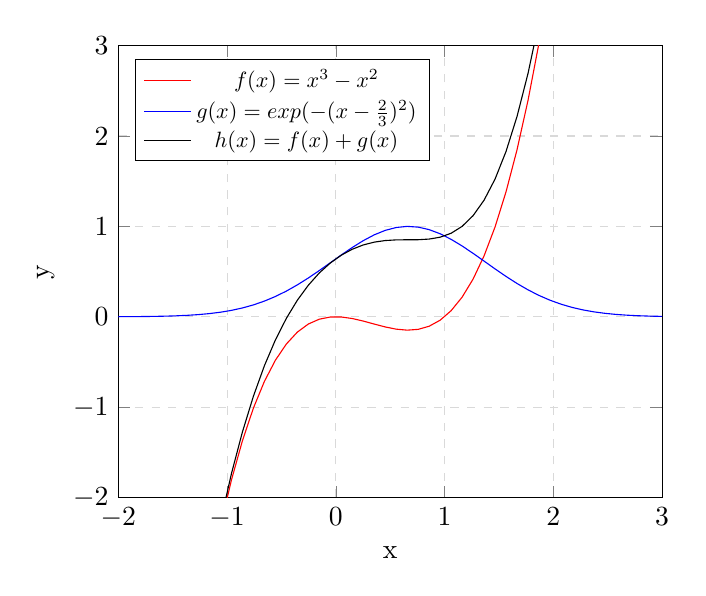
\begin{tikzpicture}
            \begin{axis}[
            grid=major, 
            grid style={dashed,gray!30},
            xlabel=x, % Set the labels
            ylabel=y,
            xmin=-2,
            xmax=3,
            xtick={-2,-1,0,1,2, 3},
            ymin=-2,
            ymax=3,
            samples=100,
            legend pos = north west,
            width=0.7\textwidth,
            legend style={nodes={scale=0.8, transform shape}}]
            \addplot[color=red]{x^3-x^2};
            \addlegendentry{$f(x)=x^3-x^2$}
            \addplot[color=blue]{exp(-(x-2/3)^2)};
            \addlegendentry{$g(x)=exp(-(x-\frac{2}{3})^2)$}
            \addplot[color=black]{x^3-x^2+exp(-(x-2/3)^2)};
            \addlegendentry{$h(x)=f(x)+g(x)$}
            \end{axis}
         \end{tikzpicture}
        \caption{Example of a function with a local minimum at $x=\frac{2}{3}$. If we place an Gaussian function on top, the minimum disappears. Note, that the black function approaches the red if we distance from the local minimum.}
    \end{center}
\end{figure}

Formally, this hill is realised by first computing the distance of the parameter
values to the checkpoint, and then adding a penalty for small distances. If we
use and exponential Kernel, the idea of the hill can be taken quite visually.
Section \ref{sub:Mathematical_approach} describes the mathematical approach in
detail.

What happens when our penalty hill is not large enough to get the ball over the
hill? This means we would get back to the present parameter values. That's not
necesarryly a problem, as it would mean that our current position is very
robust, which would lead to a good generalization capability. Therefore our
network would stay in areas with stable minima, which is a desired property.

For ensemble methods, there are other possible benefits of this approach. Recall
that for an ensemble to perform well, the errors of the participating networks
should be uncorellated. SGD with warm restart \cite{loshchilov2016sgdr} tried to
ensure this with warm restarts, where a high learnin rate increases the distance
of the networks and therefore leads to uncorellated errors. We could use our
method as alternative approach, where we ensure the distance between the
networks not only by high learning rate but by explicitly increasing the
distance. Of course, the underlying idea for both is that networks which are
more distant in parameter space will behave more differently, and therefore have
more uncorellated errors.



\subsection{Mathematical approach}\label{sub:Mathematical_approach}
\subsubsection{Distance function}\label{distance_function}
As we want to measure the distance between two points, we need to define a
distance function. A common choice is the euclidean distance also know as $L_2$
norm, which is defined as: 
\begin{align}
    \rVert x \lVert_2 = \sqrt{\sum_i \lvert x_i \rvert^2}
\end{align}
This norm can also be squared to get rid of the root. Squaring does not change
the direction of the gradient, and is therefore possible. To measure the
distance between two parameter states $\theta_1$ and $\theta_2$ of the networks,
this results in:
\begin{align}\label{eq:distance}
    L_2 (\theta_1, \theta_2)= \sum_i (\theta_{1_i}-\theta_{2_i})^2
\end{align}
The size and shape of the paramters $\theta$ is not important, as each paramter
is only compared to another state of itself, and is combined via a sum.

An undesireable property of the current formulation is that the values the
distance function can take is partly dependend on the size of the network.
Consider two networks $\theta_1$, $\theta_2$ with the same classification task,
but the number of parameters of $\theta_1$ is larger than $\theta_2$ If we
assume all of the parameters are distributed the same way, then $\theta_1$ would
output a larger distance than $\theta_2$. However it would be desirable for the
functions to be in the same bound, as it would make the transfer of
hyperparameters for example possible. That's why we need a function to let the
output stay in a certan bound.

If we take a look at support vector machines, they use kernels to compute the
similarity between two samples. One popular choice is the radial basis function
kernel, defined as:
\begin{align}\label{eq:RBF}
    k(\theta_1, \theta_2)=exp(-\frac{\rVert \theta_1 - \theta_2 \lVert^2}{\sigma^2})
\end{align}
where $exp$ is the exponential function. With the use of \ref{eq:distance}, we
can convert this to:
\begin{align}\label{eq:DistanceFinal}
    distance(\theta_1, \theta_2)=exp(-\frac{L_2 (\theta_1, \theta_2)}{\sigma^2})
\end{align}

If we plot this function in the two dimensional case in figure
\ref{fig:Gaussian}, we can see some nice properties. First of all, the values
are now bound between 0 an 1, regardless of the size of $\theta$. Second, we can
see as the values of the distance get larger, the function approaches 0
asymtotically. This leads to a really small gradient for extreme distances.
Consequently, the Kernel will initially push the parameters away from the
checkpoint, but when this is achieved, will have little influence on the loss
function. How far the function encourages to distance from the checkpoint can be
controlled by the parameter $\sigma$, which defines the width of the function
and can be tuned as a hyperparamter. As $\sigma$ gets larger, the function
becomes wider. Therefore, the influence of the distance function will reach
further the larger $\sigma$ is.

\begin{figure}[h]\label{fig:Gaussian}
    \centering
    \begin{center}
        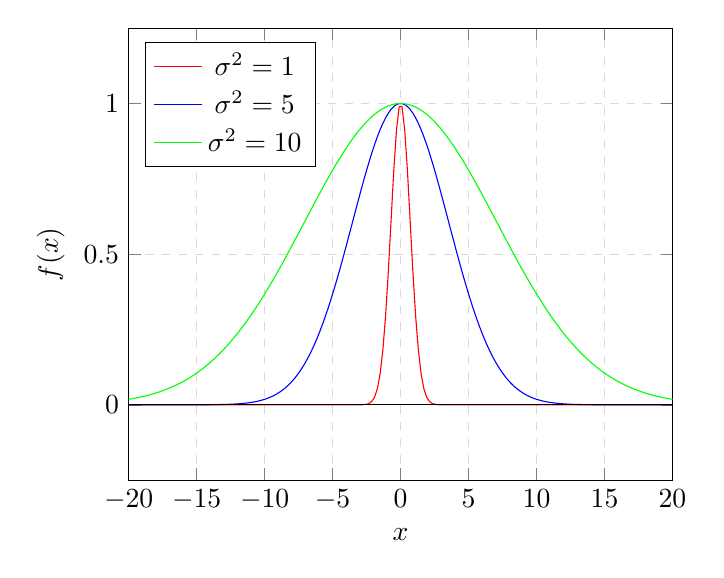
\begin{tikzpicture}
            \begin{axis}[
            grid=major, 
            grid style={dashed,gray!30},
            xlabel=$x$, % Set the labels
            ylabel=$f(x)$,
            xmin=-20,
            xmax=20,
            xtick={-20,-15,-10,-5,0,5,10,15,20},
            ytick={0,0.5,1},
            ymin=-0.25,
            ymax=1.25,
            samples=200,
            legend pos = north west,
            width=0.7\textwidth,
            legend style={nodes={scale=1, transform shape}},
            domain=-20:20]
            \addplot[color=red]{exp(-x^2)};
            \addlegendentry{$\sigma^2=1$}
            \addplot[color=blue]{exp(-x^2/5^2)};
            \addlegendentry{$\sigma^2=5$}
            \addplot[color=green]{exp(-x^2/10^2)};
            \addlegendentry{$\sigma^2=10$}
            \addplot[color=black]{0};
            \end{axis}
         \end{tikzpicture}
         \caption{Plot of the function $f(x)=exp(-\frac{x^2}{\sigma^2})$ for different values of $\sigma^2$.}
    \end{center}
\end{figure}


\subsubsection{Loss function}\label{sub:Loss_function}
The last section has focused on how to implement a loss function which achieves
distancing from parameter values. However, only using this loss function would
sacrafice network performance. Therefore, we combine it with the standard loss
function of the task. The state of the art loss function for image
classification, which will be used for testing later, is the cross-entropy-loss
defined as:
\begin{align}
    -\sum_{i} \delta_{yc} log(f(x)_i)
\end{align}
Where $\delta$ is the Kronecker-Delta function defined as:
\begin{align}
    \delta_{xy} =
    \begin{cases}
        1 \textrm{, if } x=y \\
        0 \textrm{ otherwise}
    \end{cases}
\end{align}

To account for the distance term, we just sum it with the cross-entropy-loss:
\begin{align}\label{eq:Loss_distance}
    L=\sum_{i} \delta_{yi} log(f(x)_i) + distance(\theta, \theta_c)
\end{align}
Where $\theta_c$ is the checkpoint. Note that we can do this multiple times, so
we can incooperate multiple checkpoints. Here, we divide by the number of
checkpoints to keep the influence of the distance function on the loss function
irrelevant of the number of checkpoints.
\begin{align}
    L=\sum_{i} \delta_{yi} log(f(x)_i) + \frac{1}{c} \sum_c distance(\theta, \theta_c)
\end{align}
When computing the derivative for the backpropagation, the sum
decomposes into two terms, so the cross-entropy-loss will be computed the same
as before. Another property we want to control for is the influence of the
distance versus the cross-entropy-loss. When training is in later stages, the
cross-entropy-loss may be very small. If the values of the distance function a
too large in comparison, this would cause the parameters to be updated only
based on the distance, which is undesirable as the performance wouldn't be taken
into account anymore. The same is also true the other way around, if the
distance function is too small, it wouldn't affect training at all. That's why
we introduce a hyperparameters $s$ called strength to control this:
\begin{align}\label{eq:Loss_strength}
    L=\sum_{c} \delta_{yc} log(f(x)_c) + s \cdot distance(\theta, \theta_c)
\end{align}
Figure \ref{fig:Gaussian_strength} shows the infuence of $s$ on the distance
function. The values are now bound between 0 and $s$. Increasing the strength
also has the same effect of the function getting wider as in figure
\ref{fig:Gaussian}, but at a much smaller scale. 

\begin{figure}[h]\label{fig:Gaussian_strength}
    \centering
    \begin{center}
        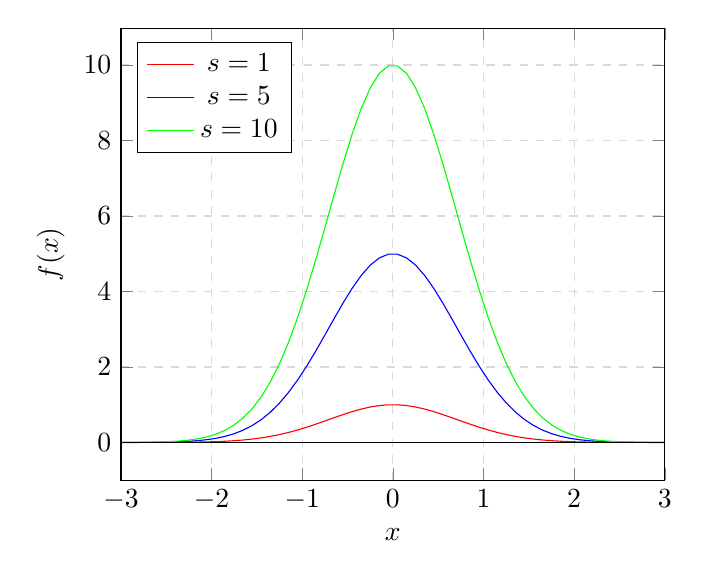
\begin{tikzpicture}
            \begin{axis}[
            grid=major, 
            grid style={dashed,gray!30},
            xlabel=$x$,
            ylabel=$f(x)$,
            xmin=-3,
            xmax=3,
            %xtick={-5,-1,0,1,5},
            %ytick={0,1,5,10},
            %ymin=-1,
            %ymax=11,
            samples=400,
            legend pos = north west,
            width=0.7\textwidth,
            legend style={nodes={scale=1, transform shape}},
            domain=-20:20]
            \addplot[color=red]{exp(-x^2)};
            \addlegendentry{$s=1$}
            \addplot[color=blue]{5*exp(-x^2)};
            \addlegendentry{$s=5$}
            \addplot[color=green]{10*exp(-x^2)};
            \addlegendentry{$s=10$}
            \addplot[color=black]{0};
            \end{axis}
         \end{tikzpicture}
         \caption{Plot of the function $f(x)=s\cdot exp(-\frac{x^2}{\sigma^2})$ for different values of $s$.}
    \end{center}
\end{figure}

\subsubsection{Effect on Gradient}\label{sub:Effect_on_Gradient} 
In section \ref{sub:Loss_function}, we showed how the new loss function is
composed. The normal cross-entropy-loss and the distance function are added
together. Therefore, taking the derivative of equation \ref{eq:Loss_distance}
results in 
\begin{align}
    \nabla_\theta L 
    &= \nabla_\theta (\sum_{i} \delta_{yi} log(f(x)_i) + distance(\theta, \theta_c))\\
    &= \nabla_\theta (\sum_{i} \delta_{yi} log(f(x)_i)) + \nabla_\theta distance(\theta, \theta_c)
\end{align}
The derivative of the sum decomposes in the sum of the derivatives. Therefore,
the cross-entropy-loss will be added to the gradient the same as before. The new
term is the distance function on the right.

First of all, it influences the direction of the gradient, so that the network
parameters distance from their checkpoint values. If we take one parameter
$\theta_i$ and compute the derivative of the distance function with respect to
the checkpoint $\theta_c$, we end up with:
\begin{align}
    \nabla_{\theta_i} distance(\theta_c, \theta_i)
    &= \nabla_{\theta_i} exp(-\frac{\sum_j (\theta_{c_j}-\theta_{j})^2}{\sigma^2}) \\
    &= \nabla_{\theta_i} (-\frac{\sum_j (\theta_{c_j}-\theta_{j})^2}{\sigma^2}) \cdot exp(-\frac{\sum_j (\theta_{c_j}-\theta_{j})^2}{\sigma^2}) \\
    &= -\frac{1}{\sigma^2} \cdot \nabla_{\theta_i} \sum_j (\theta_{c_j}-\theta_{j})^2 \cdot exp(-\frac{\sum_j (\theta_{c_j}-\theta_{j})^2}{\sigma^2}) \\
    &= -\frac{1}{\sigma^2} \cdot 2 (\theta_{c_i} - \theta_i) \cdot \nabla_{\theta_i}(\theta_{c_i} - \theta_i) \cdot exp(-\frac{\sum_j (\theta_{c_j}-\theta_{j})^2}{\sigma^2}) \\
    &= -\frac{1}{\sigma^2} \cdot 2 (\theta_{c_i} - \theta_i) \cdot (-1) \cdot exp(-\frac{\sum_j (\theta_{c_j}-\theta_{j})^2}{\sigma^2}) \\
    &= \frac{2}{\sigma^2} \cdot (\theta_{c_i} - \theta_i) \cdot exp(-\frac{\sum_j (\theta_{c_j}-\theta_{j})^2}{\sigma^2}) 
\end{align}

Only the factor $(\theta_{c_i} - \theta_i)$ will affect the direction of the
gradient, the other terms will be $>=0$ for $\forall \theta_i , \theta_{c_i}\in
\mathbb{R}$ and only scale the size. Therefore, they can be disregarded and
there are three cases:
\begin{itemize}
    \item $\theta_{c_i} > \theta_i$\\
        It follows that $\nabla_{\theta_i} distance(\theta_{c_i}, \theta_i)$
        will be positive. As we apply the negative gradient to update the
        parameters, $\theta_i$ will get smaller and  $(\theta_{c_i} - \theta_i)^2$
        will be increase.
    \item $\theta_{c_i} < \theta_i$\\
        $\nabla_{\theta_i} distance(\theta_{c_i}, \theta_i)$ will be negative
        and the distance $(\theta_{c_i} - \theta_i)^2$ will increase the same as
        above.
    \item $\theta_{c_i} = \theta_i$\\
        $\nabla_{\theta_i} distance(\theta_{c_i}, \theta_i)$ will be 0.
        Therefore, the parameter value $\theta_i$ will stay the same.
\end{itemize} 

For $\theta_{c_i} \neq \theta_i$, the gradient of the distance function will
successfully increase the distance. For $\theta_{c_i} = \theta_i$ however, it
will introduce no gradient at all. This would problematic, as when a checkpoint
is created, before the first update this case is true. However, the update is
also composed of the cross-entropy-loss, which will likely introduce an non-zero
gradient. In the next iteration, $\theta_{c_i} \neq \theta_i$ will then be true
and the distance function works as expected. If Momentum is used, there is
another term that prevents the gradient from becoming 0.


Besides the influence of the distance function on the direction of the gradient,
we expect an influence size of the gradient. Assume that the direction of the
gradient is stable across multiple iterations, which is likely if we use
Momentum. After we create a checkpoint, the normal loss function would therefore
increase the distance to the checkpoint by itself. As we have seen above, the
gradient of the distance function will also increase the distance, therefore
both gradients will point in the same direction. For a stable gradient direction
of the normal loss function, the distance function therefore increases the
gradient size rather than change the gradient orientation. Only when the
direction for a parameter changes, the distance term will work against it.

\subsubsection{Computational analysis}\label{sub:Computational_Analysis}
Although the network performance is one of the most important aspects of a
neural network, other factors like training time have to be taken into account.
Here, we will analyze how the distance term affects training time. Algorithm
\ref{alg:Checkpoint} shows that at the beginning, the network is trained as
usual. Therefore, there is no additional training time in this stage. After we
add the checkpoint however, the distance function is added to the loss. In
section \ref{sub:Effect_on_Gradient} we have seen that there is no interaction
between the gradient of the cross-entropy-loss and the distance function. The
same is true for the foward pass. Therefore, the only added computation time
raises from the distance term itself.

The number of parameters of the network stays constant over the epochs.
Therefore, the number of mathematical operations in the foward and backward pass
of the distance term stays constant. Lets assume the comparison time for two
numbers is also constant regardless of their size. Then it follows, that the
distance function creates a constant additional amount of time, denotet by $d$.
In addition, let $l$ denote the constant cost of one pass trough the regular
training loop. If we pass this loop $n$ times, our inital cost is $O(l\cdot
n)=O(n)$. If we add our distance function, we have to add $O(n\cdot d)$ to our
cost $O(n\cdot l + n \cdot d)$. As $O(n\cdot l + n \cdot d)=O(n\cdot (l +
d))=O(n)$, the complexity of the algorithm stays the same. However, the distance
function will still raise the per epoch cost, although by a constant. If we add
more checkpoints, there are again no interactions with other checkpoints or the
regular training loop. Therefore, every new checkpoint should add the same
additional cost, while keeping the complexity class the same. The actual value
of the additional cost will be discussed in the results, section
\ref{Res:Computational_cost}.


\subsection{Pytorch implementation}

\subsubsection{Checkpoint creation}
To measure the distance, we have to create the checkpoint. The model parameters
in pytorch are stored as matrices for each layer and can be accesed via
$model.parameters()$, which outputs an iterable. We therefore opt to keep this
structure and safe the parameters in a list.
\begin{algorithm}[h!]
    \caption{Checkpoint}\label{alg:Checkpoint}
    \lstset{language=Python}
    \lstinputlisting{src/createCheckpoint.py}
\end{algorithm}
\newline
First, the checkpoint list is initialized. Then we iterate over the model
parameters. For each layer, we have to clone the parameters in order to create
new variables, and not just pointers to the existing ones. In addition they have
to be detached, to remove connection of the gradient to the model parameters.

\subsubsection{Distance function}
The L2 norm is implemented the follwing way: We iterate over the checkpoint and
the current parameter values. For each layer, we compute the difference, and
then square and add the values to our distance.
\begin{algorithm}[h!]
    \caption{L2 norm}\label{alg:L2Norm}
    \lstset{language=Python}
    \lstinputlisting{src/L2.py}
\end{algorithm}

\subsubsection{Loss function}
Finally, we add our distance term and the regular loss function together. First,
the standard loss is computed. Then, we iterate over all checkpoints and add
their resulting distance values to the loss.
\begin{algorithm}[h!]
    \caption{Loss function}
    \lstset{language=Python}
    \lstinputlisting{src/loss_distance.py}
\end{algorithm}



\section{Configuration}

\subsection{Library and Training}
The code for the network was written in Python 3.7.4 , with the use of Pytorch
\cite{NEURIPS2019_9015} as the machine learning library. Data that occured
during training was logged and plotted with Tensorboard. Training was done on
the TCML Cluster of the University of Tübingen \cite{TCML}.

\subsection{Dataset}
CIFAR-10 \cite{CIFAR-10} is a popular dataset for image classification. It
consists of 60000 32x32 colour images with 10 different classes. The dataset is
seperated into 50000 train and 10000 test images. The state of the art accuracy
is 97.3\%, reported from Kolesnikov et al. \cite{kolesnikov2019big}.

The data is tranformed by using a random crop, random horizontal flip and
normalization.


\subsection{Networks}
\subsubsection{ResNet}\label{sub:ResNet}
The Residual Network (ResNet) architecture was first proposed by He et al.
\cite{he2016deep}. The idea of the ResNet was, that it is more easy for a
network to learn the residuals rather than the full transformation of an input.
Formally, consider the input $x$. The network transforms $x$ accoring to $H(x)$.
Rather than letting the network do the full transformation, ResNet produces
$H(x)= x +f(x)$, where $f(x)$ is the residual transformation learned by the
network, and x the identity data which is realized by a skip connection. Figure
\ref{fig:Residual_Block} shows a graphical illustration. Beside the assumably
easier to learn representation, ResNet also solves other problems. The issue of
the vanishing gradient as discussed in section \ref{sub:Vanishing_gradient} for
example is tackled, as skip connections backpropagate the gradient better to
earlier layers of the network. This allows for deeper networks.

\begin{figure}[h]\label{fig:Residual_Block}
    \centering
    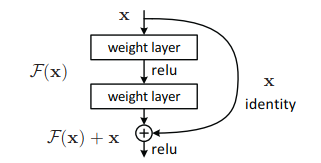
\includegraphics[width=0.6\textwidth]{images/Residual_Block.png}
    \caption{Residual Block from \cite[Page 2]{he2016deep}}
\end{figure}

ResNet creates basic building blocks by applying a convolution, a Relu and
another convolution before adding the skip connection with a final Relu. Figure
\ref{fig:Residual_Block} illustrates this block. The blocks are then stacked
after each other. To let the network learn a more complex representation, after
a number of block, they increase the number of channels. Here, the identity
mapping of the skip connection is replaced by a pointwise convolution to
increase the number of channels. Alternatively, the new channels are padded with
0.



\subsubsection{MobileNetV2}
MobileNet was first introduced by Howard et. al \cite{howard2017mobilenets} as a
lightweight neural network for the use on mobile devices. To reduce the
computation effort of the network, they made use of the depth-wise seperable
convolution. Consider a 32x32x3 image of the CIFAR-10 dataset. A traditional 3x3
convolution with a stride and padding of 1 would produce an output of the shape
32x32x1. To get more channels, we would need more kernels. For a total of $k$
output channels, we would need to perform $32\cdot 32 \cdot k=1024\cdot k$
convolutions, where each convolution with the Kernel has $3\cdot 3 \cdot 3=27$
multiplications, resulting in a total of $27648\cdot k$ multiplications.
Instead of doing the computation in one kernel, depth-wise seperable convolution
divides it into two kernels. First they perform a depthwise convolution, where a
kernel of 3x3x1 is applied to every channel of the input, so in this case we end
up same size of 32x32x3. To get to k channels, they use a pointwise convolution
across the channels. This is a 1x1x3 convolution, which upscales the image to
more channels. So if we want k output channels, we need k 1x1x3 kernels. The
benefit of this technique is that, while getting the same output size, we only
need $32\cdot 32 \cdot 3=3072$ convolutions of a $3\cdot 3=9$ Kernel, resulting
in 27648 multiplications. In the second step, we need $32\cdot 32\cdot
k=1024\cdot k$ convolutions of a Kernel with $1\cdot 1\cdot 3=3$ multiplications
resulting in $3027\cdot k$ convolutions. This results in a total of $27648 +
3027\cdot k$ convolutions. Although this might be more for $k=1$, it scales up
way smaller for larger $k$, because of the number of channels only be dependend
on the lightweight pointwise convolution. For example for $k=10$, depthwise
seperable only needs 57918 multiplications while a traditional convolution needs
276480. Figure \ref{fig:DSConv} shows a graphical illustration of this idea.
\begin{figure}[h!]\label{fig:DSConv}
    \centering
    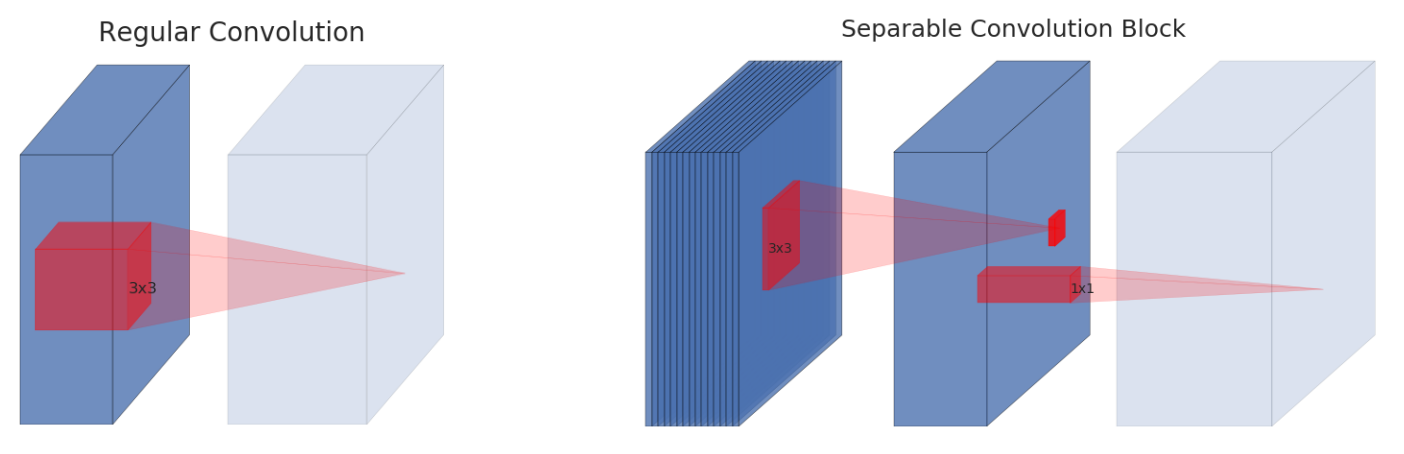
\includegraphics[width=0.6\textwidth]{images/Depthwise_Separable_Convolution.png}
    \caption{Depthwise Separable Convolution from \cite[Page 3]{sandler2018mobilenetv2} \newline On the left,
     a regular convolution with a 3x3xDepth kernel is drwan. On the right, this
     convolution is separated in depthwise convolution with a 3x3x1 Kernel,
     followed by a pointwise convolution with a 1x1xDepth Kernel. This methods
     saves computation time over the standard method, while also allowing
     interactions between channels.}
\end{figure}


With the second iteration called MobileNetV2 \cite{sandler2018mobilenetv2}, they
added the concept of inverted residuals or as they call it bottlenecks. The
ideas is, that intermediate representations should be low rather than high
dimensional. The bottleneck layer starts with a matrix with a small number of
depth channels. In the first step, the representation is expanded by a pointwise
convolution, followed by a Relu6. The expansion factor here controls how much
channels the intermediate representation will have. Then a depthwise convolution
is applied as an transformation step, followed again by a Relu6. Finally, a
pointwise convolution is applied again, but this time without a nonlinear
transformation following afterwards. The idea is that when compressing the data
back to a low dimensional space, a nonlinearity would only lead to a loss of
information. Finally, a skip connection from the input to the output is applied
to get a residual mapping from input to output.

For ImageNet, MobileNetV2 reaches an top-1 accuracy of 72\%, which outperforms
the competitors like MobileNetV1 or ShuffleNet 1.5 while having a similar number
of parameters.


\begin{figure}[h]\label{fig:InvRes}
    \centering
    \includegraphics[width=0.6\textwidth]{images/Inverted_Residual.png}
    \caption{Inverted Residual Block from \cite[Page 3]{sandler2018mobilenetv2}\newline 
    First, a Relu 6 followed by a Pointwise Convolution is applied to map the
     data to a higher dimensional space. Then a depthwise convolution is
     applied, followed again by a Relu6. Finally, the data is compressed back to
     the original size. This time, there is no Relu applied to avoid the loss of
     information.}
\end{figure}


\subsection{Network hyperparameters and training loop}\label{sub:Hyperparameters}
For both networks, the base hyperparameters are the same. Note that these
parameters are only standard configurations and may be changed to investigate
the effects:
\begin{itemize}
    \item Optimization Algorithm \\Stochastic Gradient descent combined with
    Momentum is used. A $\lambda$ of 0.9 is set for Momentum.
    \item Learning rate \\Initially 1e-2
    \item Batch size \\128
    \item Regularization \\An $L_2$ Regularization as described in chapter
    \ref{sub:Generalization} is used with a factor of 1e-3.
    \item Loss Function \\Cross-Entropy Loss
    \item Number of epochs \\The number of epochs varies. As this is an
    explorative analysis, the training is often run for a large number of
    epochs, to investigate long term changes. Usually an epoch number of 600 is
    used.
\end{itemize}


\chapter{Results}
Even with such a simple formulation, there are many different variations that
can be tested. First is the influence of the strength and width parameter of the
distance function, which will be tested in section \ref{res:Hyperparameters}. We
will also briefly test different kernels besides the RBF Kernel from equation
\ref{eq:RBF} in section \ref{res:Kernel}. In section \ref{res:Multiple}, we will
use more than one checkpoint and will also try to combine these to a global one.
The interaction of training hyperparameters like learning rate and epochs will
be discussed in section \ref{res:Training}. Finally, the usage for ensemble
methods will be tested.

\section{Baseline}
For the baseline, we use the hyperparameters as defined in section
\ref{sub:Hyperparameters}. Figure \ref{fig:Results_baseline} shows the result,
if we add a checkpoint after 100 epochs of training. For the validation accuray,
we can see that it stays similar to the accuracy without the distance function.
If we plot the distance the network gets to the checkpoint however, we can see
that the network trained with distance function clearly increases its distance
more than the one trained without. Furthermore, the red plot follows the shape
we would expect from the distance function. At the beginning, the distance
increases relatively fast, as can be expected from the high gradient of the RBF
Kernel. But as the distance increases, its gradient becomes smaller, similar to
the gradient of the Kernel. The blue plot in contrast follows an almost linear
curve, whith a much smaller gradient. Therefore, the additional term succeeds in
the initial goal, which was to distance from the checkpoint. Note that despite
the validation accuracy beeing in an area of convergence, SGD even without
distance function keeps on walking and never truly stops at a point.

\begin{figure}[h]\label{fig:Results_baseline}
    \begin{center}
        \begin{tikzpicture}
            \begin{groupplot}[
                group style={
                group size=2 by 2,
                horizontal sep=10pt,
                vertical sep=10pt,
                group name=G},
                width=8cm,
            ]

            \nextgroupplot[
            grid=major, 
            grid style={dashed,gray!30},
            % xlabel=Epoch,
            ylabel=Validation Accuracy,
            xticklabels={,,},
            ymin=0.8,
            xmin=-10]
            \addplot[mark=None, color=red] 
                table[x=Step, y=Value, col sep=comma]{images/network_csv/baseline/baseline/MobileNetV2_baseline_validation_acuracy.csv};
            \addplot[mark=None, color=blue] 
                table[x=Step, y=Value, col sep=comma]{images/network_csv/baseline/baseline_distance/MobileNetV2_baseline_distance_validation_acuracy.csv};
            
            \nextgroupplot[
                grid=major, 
                grid style={dashed,gray!30},
                % xlabel=Epoch,
                ylabel=Distance,
                yticklabel pos=right,
                xticklabels={,,},
                ylabel near ticks]
                \addplot[mark=None, color=red] 
                    table[x=Step, y=Value, col sep=comma]{images/network_csv/baseline/baseline/MobileNetV2_baseline_distance0.csv};
                \addplot[mark=None, color=blue] 
                    table[x=Step, y=Value, col sep=comma]{images/network_csv/baseline/baseline_distance/MobileNetV2_baseline_distance_distance0.csv};
    

            \nextgroupplot[
            grid=major, 
            grid style={dashed,gray!30},
            xlabel=Epoch, % Set the labels
            ylabel=Validation Accuracy,
            ymin=0.8,
            xmin=-10]
            \addplot[mark=None, color=red] 
                table[x=Step, y=Value, col sep=comma]{images/network_csv/baseline/baseline/ResNet32_baseline_validation_acuracy.csv};
            \addplot[mark=None, color=blue] 
                table[x=Step, y=Value, col sep=comma]{images/network_csv/baseline/baseline_distance/ResNet32_baseline_distance_validation_acuracy.csv};
            
            \nextgroupplot[
                grid=major, 
                grid style={dashed,gray!30},
                xlabel=Epoch, % Set the labels
                ylabel=Distance,
                yticklabel pos=right,
                ylabel near ticks]
                \addplot[mark=None, color=red] 
                    table[x=Step, y=Value, col sep=comma]{images/network_csv/baseline/baseline/ResNet32_baseline_distance0.csv};
                \addplot[mark=None, color=blue] 
                    table[x=Step, y=Value, col sep=comma]{images/network_csv/baseline/baseline_distance/ResNet32_baseline_distance_distance0.csv};

            \end{groupplot}
        \end{tikzpicture}
        \caption{Validation accuray and Distance for MobileNetV2 (upper) and ResNet32 (lower) trained without distance function (red) and with distance function (blue).}
    \end{center}
\end{figure}


[TODO: add gradient size to show that circular path]




\section{Distance function Hyperparameters}\label{res:Hyperparameters}
\subsection{strength}
Recall section \ref{eq:Loss_strength}, where we added strength as a
hyperparameter, controlling the influence of the distance function. As the RBF
Kernel is bound between 0 and 1, the strength hyperparameter will increase that
bound between 0 and the strength value.

For higher strength values, the validation accuracy receives an initial drop,
which is larger the higher the strength parameter value. This may be due to the
increased influence of the strength function. Each distance between the
parameters and the checkpoint starts at 0, therefore the values of the
exponential function starts at $strength \cdot 1$. A higher strength value will
lead to a higher influence on the loss function, and consequently the gradient.
The gradient of the cross-entropy loss will be insignificant, and the optimizer
will update the weights without regards to the validation accuracy, hence the
drop at the beginning. The distance plot reflects this behaviour, as we can see
an larger increase in distance for larger strength values. [add from wedge paper]

After the initial step however, the distance quickly converges. This is due to
the fact that after the initial increase, the value of the Kernel quickly
reaches 0. [TODO: Sow plot of strength]. Therefore, the distance Kernel becomes
insignificant again, and the Cross-Entropy loss is followed. The validation
accuracy reflects this behaviour, as after the initial drop the accuracy
recovers to the level of before. This provides additional insight in the loss
landscape. As the network distances from it`s current position on the loss
landscpae, but is still able to reach high accuracy, there have to be areas of
high accuracy everywhere on the landscape. This is in consonance to other
research in this field, as discussed in section \ref{loss_landscape}.

As a result, the value of the strength doesn't matter in long term at least. It
merely increases the distance to the checkpoint by defining how long the
distance term is important to the loss function. But after that, the normal loss
is followed again. As the last section and literature suggests, area of low loss
and high accuray can be found everywhere. Therefore, the same accuracy as before
can be reached, no matter the value of the strength. On the other hand, it is
also unlikely that it will outperform the last best value, as new areas are not
generally better than other.

basic results:
- if higher strength factor, distance rises more quickly
- then stays in this area of distance
- validation accuracy drops because first influenence of distance




\begin{figure}[h]\label{fig:Results_strength}
    \begin{center}
        \begin{tikzpicture}
            \begin{groupplot}[
                group style={
                group size=2 by 2,
                horizontal sep=10pt,
                vertical sep=10pt,
                group name=G},
                width=8cm
            ]

            \nextgroupplot[
            grid=major, 
            grid style={dashed,gray!30},
            % xlabel=Epoch,
            y label style={at={(axis description cs:0.1,0)},anchor=south},
            ylabel=Validation Accuracy,
            xticklabels={,,},
            ymin=0.6,
            legend pos= south east,
            xmin=-10]
            \addplot[mark=None, color=red] 
                table[x=Step, y=Value, col sep=comma]{images/network_csv/strength/MobileNetV2/MobileNetV2_strength_e1_validation_acuracy.csv};
            \addlegendentry{$s=0.1$}
            \addplot[mark=None, color=blue] 
                table[x=Step, y=Value, col sep=comma]{images/network_csv/baseline/baseline_distance/MobileNetV2_baseline_distance_validation_acuracy.csv};
            \addlegendentry{$s=1$}
            \addplot[mark=None, color=orange] 
                table[x=Step, y=Value, col sep=comma]{images/network_csv/strength/MobileNetV2/MobileNetV2_strength_e2_validation_acuracy.csv};
            \addlegendentry{$s=10$}
            \addplot[mark=None, color=green] 
                table[x=Step, y=Value, col sep=comma]{images/network_csv/strength/MobileNetV2/MobileNetV2_strength_e3_validation_acuracy.csv};
            \addlegendentry{$s=100$}

            \nextgroupplot[
                grid=major, 
                grid style={dashed,gray!30},
                % xlabel=Epoch,
                % y label style={at={(axis description cs:0.,0)},anchor=south},
                ylabel=Distance,
                yticklabel pos=right,
                xticklabels={,,},
                ylabel near ticks]
            \addplot[mark=None, color=red] 
                table[x=Step, y=Value, col sep=comma]{images/network_csv/strength/MobileNetV2/MobileNetV2_strength_e1_distance0.csv};
            \addplot[mark=None, color=blue] 
                table[x=Step, y=Value, col sep=comma]{images/network_csv/baseline/baseline_distance/MobileNetV2_baseline_distance_distance0.csv};
            \addplot[mark=None, color=orange] 
                table[x=Step, y=Value, col sep=comma]{images/network_csv/strength/MobileNetV2/MobileNetV2_strength_e2_distance0.csv};
            \addplot[mark=None, color=green] 
                table[x=Step, y=Value, col sep=comma]{images/network_csv/strength/MobileNetV2/MobileNetV2_strength_e3_distance0.csv};
    

            \nextgroupplot[
            grid=major, 
            grid style={dashed,gray!30},
            % x label style={at={(axis description cs:1.5,0)},anchor=west},
            xlabel=Epoch, % Set the labels
            % ylabel=Validation Accuracy,
            ymin=0.6,
            xmin=-10]
            \addplot[mark=None, color=red] 
                table[x=Step, y=Value, col sep=comma]{images/network_csv/strength/ResNet32/ResNet32_strength_e1_validation_acuracy.csv};
            \addplot[mark=None, color=blue] 
                table[x=Step, y=Value, col sep=comma]{images/network_csv/baseline/baseline_distance/ResNet32_baseline_distance_validation_acuracy.csv};
            \addplot[mark=None, color=orange] 
                table[x=Step, y=Value, col sep=comma]{images/network_csv/strength/ResNet32/ResNet32_strength_e2_validation_acuracy.csv};
            \addplot[mark=None, color=green] 
                table[x=Step, y=Value, col sep=comma]{images/network_csv/strength/ResNet32/ResNet32_strength_e3_validation_acuracy.csv};
            
            \nextgroupplot[
                grid=major, 
                grid style={dashed,gray!30},
                %xlabel=Epoch, % Set the labels
                %ylabel=Distance,
                yticklabel pos=right,
                ylabel near ticks]
            \addplot[mark=None, color=red] 
                table[x=Step, y=Value, col sep=comma]{images/network_csv/strength/ResNet32/ResNet32_strength_e1_distance0.csv};
            \addplot[mark=None, color=blue] 
                table[x=Step, y=Value, col sep=comma]{images/network_csv/baseline/baseline_distance/ResNet32_baseline_distance_distance0.csv};
            \addplot[mark=None, color=orange] 
                table[x=Step, y=Value, col sep=comma]{images/network_csv/strength/ResNet32/ResNet32_strength_e2_distance0.csv};
            \addplot[mark=None, color=green] 
                table[x=Step, y=Value, col sep=comma]{images/network_csv/strength/ResNet32/ResNet32_strength_e3_distance0.csv};

            \end{groupplot}
        \end{tikzpicture}
        \caption{Validation accuray and Distance for MobileNetV2 (upper) and ResNet32 (lower) trained without distance function (red) and with distance function (blue).}
    \end{center}
\end{figure}

\subsection{width}
We have seen in chapter \ref{distance_function}, how the width $\sigma$
influences the distance function: The larger $\sigma$ gets, the wider it
becomes. Therefore, a larger $\sigma$ should result in the network distancing
further from it's checkpoint than for smaller values. That's exactly what can be
seen in figure \ref{}: For an $\sigma$ of 0.1, the distance follows the one of
network trained without distance function, due to the RBF Kernel quickly
becoming 0. The larger the width, the slower the values of the RBF Kernel
decrease for further distance. Therefore, the gradient of the distance function
will stay quite large, pushing the network further away. This can be seen for
higher $\sigma$ values, where the distance increases further.


Initially however, the distance plot doesn't reflect this behaviour. The curve
for $\sigma = 0.01$ has a higher distance value than for $\sigma = 0.001$.
That's because the gradient of the RBF Kernel is higher for small distances, the
smaller $\sigma$. But for larger distances, this effect flips with the gradient
of the larger width staying higher for more epochs. Therefore, the curves
intersect after additional epochs. The smaller width converges, while the larger
stays constant until eventually reaching it`s area of convergence. The
intersection happens later the larger the width, for $\sigma = 0.0001$, only
after 207 epochs.

This behaviour however has no influence on the validation accuracy, which stays
the same for every width, in contrast to the strength. This may be due to the
fact, that a larger width does in fact decreases the size of the gradient. A
smaller gradient over more epochs will be added to the gradient of the
Cross-Entropy Loss. The optimizer therefore nearly keeps on following the normal
gradient and descending the valley of low loss, with a small but steady push to
increase the distance to the checkpoint. Therefore, even if the network is
allowed to move quite freely on the loss surface, it finds areas of low loss and
high accuracy in distant areas of the checkpiont, meaning there has to be good
local minima everywhere on the landscape.

[mention witdh e-3 good behaviour in terms of tradeoff]

\begin{figure}[h]\label{fig:Results_strength}
    \begin{center}
        \begin{tikzpicture}
            \begin{groupplot}[
                group style={
                group size=2 by 2,
                horizontal sep=10pt,
                vertical sep=10pt,
                group name=G},
                width=8cm
            ]

            \nextgroupplot[
            grid=major, 
            grid style={dashed,gray!30},
            % xlabel=Epoch,
            ylabel=Validation Accuracy,
            xticklabels={,,},
            ymin=0.7,
            legend pos = south east,
            xmin=-10]
            \addplot[mark=None, color=red] 
                table[x=Step, y=Value, col sep=comma]{images/network_csv/width/MobileNetV2/MobileNetV2_width_e1_validation_acuracy.csv};
            \addlegendentry{$\sigma^2=1$}
            \addplot[mark=None, color=orange] 
                table[x=Step, y=Value, col sep=comma]{images/network_csv/width/MobileNetV2/MobileNetV2_width_e2_validation_acuracy.csv};
            \addlegendentry{$\sigma^2=10$}
            \addplot[mark=None, color=blue] 
                table[x=Step, y=Value, col sep=comma]{images/network_csv/baseline/baseline_distance/MobileNetV2_baseline_distance_validation_acuracy.csv};
            \addlegendentry{$\sigma^2=100$}
            \addplot[mark=None, color=green] 
                table[x=Step, y=Value, col sep=comma]{images/network_csv/width/MobileNetV2/MobileNetV2_width_e4_validation_acuracy.csv};
            \addlegendentry{$\sigma^2=1000$}

            \nextgroupplot[
                grid=major, 
                grid style={dashed,gray!30},
                % xlabel=Epoch,
                ylabel=Distance,
                yticklabel pos=right,
                xticklabels={,,},
                ylabel near ticks]
            \addplot[mark=None, color=red] 
                table[x=Step, y=Value, col sep=comma]{images/network_csv/width/MobileNetV2/MobileNetV2_width_e1_distance0.csv};
            \addplot[mark=None, color=orange] 
                table[x=Step, y=Value, col sep=comma]{images/network_csv/width/MobileNetV2/MobileNetV2_width_e2_distance0.csv};
            \addplot[mark=None, color=blue] 
                table[x=Step, y=Value, col sep=comma]{images/network_csv/baseline/baseline_distance/MobileNetV2_baseline_distance_distance0.csv};
            \addplot[mark=None, color=green] 
                table[x=Step, y=Value, col sep=comma]{images/network_csv/width/MobileNetV2/MobileNetV2_width_e4_distance0.csv};
    

            \nextgroupplot[
            grid=major, 
            grid style={dashed,gray!30},
            xlabel=Epoch, % Set the labels
            ylabel=Validation Accuracy,
            ymin=0.7,
            xmin=-10]
            \addplot[mark=None, color=red] 
                table[x=Step, y=Value, col sep=comma]{images/network_csv/width/ResNet32/ResNet32_width_e1_validation_acuracy.csv};
            \addplot[mark=None, color=orange] 
                table[x=Step, y=Value, col sep=comma]{images/network_csv/width/ResNet32/ResNet32_width_e2_validation_acuracy.csv};
            \addplot[mark=None, color=blue] 
                table[x=Step, y=Value, col sep=comma]{images/network_csv/baseline/baseline_distance/ResNet32_baseline_distance_validation_acuracy.csv};
            \addplot[mark=None, color=green] 
                table[x=Step, y=Value, col sep=comma]{images/network_csv/width/ResNet32/ResNet32_width_e4_validation_acuracy.csv};

            
            \nextgroupplot[
                grid=major, 
                grid style={dashed,gray!30},
                xlabel=Epoch, % Set the labels
                ylabel=Distance,
                yticklabel pos=right,
                ylabel near ticks]
            \addplot[mark=None, color=red] 
                table[x=Step, y=Value, col sep=comma]{images/network_csv/width/ResNet32/ResNet32_width_e1_distance0.csv};
            \addplot[mark=None, color=orange] 
                table[x=Step, y=Value, col sep=comma]{images/network_csv/width/ResNet32/ResNet32_width_e2_distance0.csv};
            \addplot[mark=None, color=blue] 
                table[x=Step, y=Value, col sep=comma]{images/network_csv/baseline/baseline_distance/ResNet32_baseline_distance_distance0.csv};
            \addplot[mark=None, color=green] 
                table[x=Step, y=Value, col sep=comma]{images/network_csv/width/ResNet32/ResNet32_width_e4_distance0.csv};

            \end{groupplot}
        \end{tikzpicture}
        \caption{Validation accuray and Distance for MobileNetV2 (upper) and ResNet32 (lower) trained with different widths of the distance function.}
    \end{center}
\end{figure}








results: - wider kernel leads to higher value of
distance - maybe slower due to smaller gradient - no difference in validation
accuracy - if so, should prove that in every area exists low loss regions -
accuracy doesn't decrease -> there are valleys leading away from current point
with high accuracy - 







\section{Multiple Checkpoint}\label{res:Multiple}
idea: distance from multiple rather than 1 place
\subsection{multiple}
For multiple checkpoints, we can see the same pattern as in section
\ref{res:Hyperparameters}. For low strength, we experience no effect at all. If
we increase the strength there is an initial drop in the accuracy, but with
further epochs, this recovers to the baseline accuracy. Furthermore, it even
tops the baseline, with a small but increasing margin for every restart that is
performed. The pattern is quite similar to warm restarts, where for every
restart the reached accuracy increases. For a in depth comparison, see section
\ref{res:Learning rate}.

\begin{figure}[h]\label{fig:Results_multiple}
    \begin{center}
        \begin{tikzpicture}
            \begin{groupplot}[
                group style={
                group size=2 by 1,
                horizontal sep=10pt,
                vertical sep=10pt,
                group name=G},
                width=8cm
            ]

            \nextgroupplot[
            grid=major, 
            grid style={dashed,gray!30},
            xlabel=Epoch,
            ylabel=Validation Accuracy,
            ymin=0.6,
            ymax=1,
            legend pos = south east,
            xmin=-10]
            \addplot[mark=None, color=red] 
                table[x=Step, y=Value, col sep=comma]{images/network_csv/multiple/MobileNetV2/MobileNetV2_multiple_validation_acuracy.csv};
                \addlegendentry{$s=1$}
            \addplot[mark=None, color=blue] 
                table[x=Step, y=Value, col sep=comma]{images/network_csv/multiple/MobileNetV2/MobileNetV2_multiple_f10_validation_acuracy.csv};
                \addlegendentry{$s=10$}
            \addplot[mark=None, color=green] 
                table[x=Step, y=Value, col sep=comma]{images/network_csv/multiple/MobileNetV2/MobileNetV2_multiple_f100_validation_acuracy.csv};
                \addlegendentry{$s=100$}
            
    

            \nextgroupplot[
            grid=major, 
            grid style={dashed,gray!30},
            xlabel=Epoch, % Set the labels
            yticklabels={,,},
            ymin=0.6,
            ymax=1,
            xmin=-10]
            \addplot[mark=None, color=red] 
                table[x=Step, y=Value, col sep=comma]{images/network_csv/width/ResNet32/ResNet32_width_e1_validation_acuracy.csv};
            \addplot[mark=None, color=orange] 
                table[x=Step, y=Value, col sep=comma]{images/network_csv/width/ResNet32/ResNet32_width_e2_validation_acuracy.csv};
            \addplot[mark=None, color=blue] 
                table[x=Step, y=Value, col sep=comma]{images/network_csv/baseline/baseline_distance/ResNet32_baseline_distance_validation_acuracy.csv};
            \addplot[mark=None, color=green] 
                table[x=Step, y=Value, col sep=comma]{images/network_csv/width/ResNet32/ResNet32_width_e4_validation_acuracy.csv};
            % [TODO: add ResNet Multiple]

            \end{groupplot}
        \end{tikzpicture}
        \caption{Validation accuray and Distance for MobileNetV2 (upper) and ResNet32 (lower) trained with multiple checkpoints. [TODO: add for ResNet]}
    \end{center}
\end{figure}

The influence on the distance to the checkpoints is more interesting however. In
general, an additional checkpoint seems to decrease the distance to the others.
This is quite counterintuitive at first glance. Suppose for one parameter, we
have checkpoint value $a$ and create a new one at our current value $b<a$. To
increase the distance to both, we would just have to walk in direction $c<b$. As
we have seen in previous section, this would be sufficient as areas of low error
exist everywhere. But why is the distance then decreased for our first
checkpoint? The reason might be the $L_2$ regularization, as it restricts the
weights to small sizes. At some point, it might be less costly to decrease the
weights again for a smaller $L_2$, traded off against a bit smaller distance to
other checkpoints. This restriction in weight space is probably why new terms
lead to a decrease of the distance to existing checkpoints.
[maybe long term convergence to each other]

\begin{figure}[h]\label{fig:Results_multiple_distance}
    \begin{center}
        \begin{tikzpicture}
            \begin{groupplot}[
                group style={
                group size=3 by 1,
                horizontal sep=10pt,
                vertical sep=10pt,
                group name=G},
                width=5cm
            ]

            \nextgroupplot[
            title=checkpoint 1,
            grid=major, 
            grid style={dashed,gray!30},
            %x label style={at={(axis description cs:1.5,0)},anchor=north},
            % y label style={at={(axis description cs:-0.1,.5)},rotate=90,anchor=south},
            %xlabel=Epoch,
            ylabel=distance,
            ylabel near ticks,
            ymax=8000,
            xmin=140]
            \addplot[mark=None, color=red] 
                table[x=Step, y=Value, col sep=comma]{images/network_csv/multiple/MobileNetV2/MobileNetV2_multiple_distance0.csv};
            \addplot[mark=None, color=green] 
                table[x=Step, y=Value, col sep=comma]{images/network_csv/multiple/MobileNetV2/MobileNetV2_multiple_f10_distance0.csv};
            \addplot[mark=None, color=blue] 
                table[x=Step, y=Value, col sep=comma]{images/network_csv/multiple/MobileNetV2/MobileNetV2_multiple_f100_distance0.csv};

            \nextgroupplot[
            title=checkpoint 2,
            grid=major, 
            grid style={dashed,gray!30},
            xlabel=Epoch,
            yticklabels={,,}
            ymax=8000,
            xmin=290]
            \addplot[mark=None, color=red] 
                table[x=Step, y=Value, col sep=comma]{images/network_csv/multiple/MobileNetV2/MobileNetV2_multiple_distance1.csv};
            \addplot[mark=None, color=green] 
                table[x=Step, y=Value, col sep=comma]{images/network_csv/multiple/MobileNetV2/MobileNetV2_multiple_f10_distance1.csv};
            \addplot[mark=None, color=blue] 
                table[x=Step, y=Value, col sep=comma]{images/network_csv/multiple/MobileNetV2/MobileNetV2_multiple_f100_distance1.csv};

            \nextgroupplot[
            title=checkpoint 3,
            grid=major, 
            grid style={dashed,gray!30},
            %xlabel=Epoch,
            yticklabels={,,},
            ymax=8000,
            legend pos = outer north east,
            xmin=440]
            \addplot[mark=None, color=red] 
                table[x=Step, y=Value, col sep=comma]{images/network_csv/multiple/MobileNetV2/MobileNetV2_multiple_distance2.csv};
                \addlegendentry{$s=1$}
            \addplot[mark=None, color=green] 
                table[x=Step, y=Value, col sep=comma]{images/network_csv/multiple/MobileNetV2/MobileNetV2_multiple_f10_distance2.csv};
                \addlegendentry{$s=10$}
            \addplot[mark=None, color=blue] 
                table[x=Step, y=Value, col sep=comma]{images/network_csv/multiple/MobileNetV2/MobileNetV2_multiple_f100_distance2.csv};
                \addlegendentry{$s=100$}

            \end{groupplot}
        \end{tikzpicture}
        \caption{Distance plots for MobileNetV2 (upper) and ResNet32 (lower) trained with multiple checkpoints and different strength values. [TODO: add for ResNet]}
    \end{center}
\end{figure}

In short term however, new checkpoint produce quite different influence on the
distance to existing ones. For a strength of $s=1$ we can see a slight decrease
which turns into a longer increase until the next checkpoint. For $s=10$, we an
aprupt decrease with an small peak after. For $s=100$, there only is a peak at
the beginning which quickly diminishes. Noticeable, this pattern repeats for the
other checkpoints and therefore seems unlikely to be a coincidence. The size of
these hills can be tracked to the size of the strength. Larger strength
introduces a larger gradient and therefore step size at the beginning, making
the hills larger. This doesn't explain the different orientation of these hills.
For the case of $s=100$, the initial increase of distance seems reasonable. As
the value of the distance function is not 0, the gradient should face in
direction away from the last checkpoint. A new checkpoint introduces a gradient
boost. As momentum preserves the old gradient, it will acclerate in direction
away from the first and the second checkpoint, therefore leading to a hill.

By this explanation, the pattern should repeat for the other cases however. It
may be argued, that this pattern would still exist for other values of s.
However, it is only recongnizable in the case of large s.




- only effect for larger strength
- initial decrease, similar to starts
- reaches slightly lower train loss, but not better validation accuracy
- have to take longer baseline run to see if it comes over baseline accuracy

- for new checkpoints effect on distance of current, at the moment not consistent -> has to check for average
- in general, seems like a slight decrease but same pattern again for single checkpoint, but others show same general pattern
- explanation idea: new kernel pushes gradient size -> increase or decrease (should be an icrease because momentum???)

- gradient size becomes smaller for distance term -> maybe hint that SGD wants
to stay in that area and distance term tries to push out -> gradient direction
would be interesting (but too far for this work)



- show that multiple minima all increase distance
- show how it can be merged to a large one

- increase factor to show differences, also überleitung to warm restarts
\subsection{merge}
A slightly different approach is to merge the checkpoints, described in section
\ref{sub:Multiple_checkpoints}.
[TODO: add more networks for merge]









\section{Training Hyperparameters}\label{res:Training}
\subsection{lr}\label{res:Learning rate}
\subsubsection{Scheduler}
Learning rate Scheduler were introduced in section \ref{sub:Learing_rate_decay},
where the learning rate was not held constant, but decayed over time. One futher
addition were warm restarts, where after the decay we set the learning rate back
up to the inital and repeat this cycle several times.

This procedure results in an increase of validation accuracy. We use a step
decay scheduler with $\gamma = 0.1$ for every 50 epochs, and a warm restart
after 150 epochs. Additionally, a cosine decay is used as in
\cite{loshchilov2016sgdr}. Figure \ref{fig:Results_scheduler} shows the
validation accuracy. We can see, that schedulers outperform a fixed learning
rate. Furthermore, the maximum accuracy of every cycle slightly increases, until
eventually coming to convergence. We can clearly see the warm restarts, as the
accuracy drops due to the high learning rate.

In section \ref{sub:cosine_decay}, the underlying idea leading to this
improvement was discussed: High learning rates should lead to exploration and
convergence to wider and more stable convergence.


\begin{figure}[h]\label{fig:Results_scheduler}
    \begin{center}
        \begin{tikzpicture}
            \begin{groupplot}[
                group style={
                group size=2 by 2,
                horizontal sep=10pt,
                vertical sep=10pt,
                group name=G},
                width=8cm
            ]

            \nextgroupplot[
            grid=major, 
            grid style={dashed,gray!30},
            % xlabel=Epoch,
            ylabel=Validation Accuracy,
            xticklabels={,,},
            ymin=0.75,
            legend pos = south east,
            xmin=-10]
            \addplot[mark=None, color=red] 
                table[x=Step, y=Value, col sep=comma]{images/network_csv/baseline/baseline/MobileNetV2_baseline_validation_acuracy.csv};
                \addlegendentry{fixed lr}
            \addplot[mark=None, color=green] 
                table[x=Step, y=Value, col sep=comma]{images/network_csv/scheduler/MobileNetV2/MobileNetV2_scheduler_step_validation_acuracy.csv};
                \addlegendentry{step decay}
            \addplot[mark=None, color=blue] 
                table[x=Step, y=Value, col sep=comma]{images/network_csv/scheduler/MobileNetV2/MobileNetV2_scheduler_cosine_validation_acuracy.csv};
                \addlegendentry{cosine decay}
            \nextgroupplot[
                grid=major, 
                grid style={dashed,gray!30},
                % xlabel=Epoch,
                ylabel=Distance,
                yticklabel pos=right,
                xticklabels={,,},
                ylabel near ticks]
            \addplot[mark=None, color=red] 
                table[x=Step, y=Value, col sep=comma]{images/network_csv/baseline/baseline/MobileNetV2_baseline_distance0.csv};
            \addplot[mark=None, color=green] 
                table[x=Step, y=Value, col sep=comma]{images/network_csv/scheduler/MobileNetV2/MobileNetV2_scheduler_step_distance0.csv};
            \addplot[mark=None, color=blue] 
                table[x=Step, y=Value, col sep=comma]{images/network_csv/scheduler/MobileNetV2/MobileNetV2_scheduler_cosine_distance0.csv};
    

            \nextgroupplot[
            grid=major, 
            grid style={dashed,gray!30},
            xlabel=Epoch, % Set the labels
            ylabel=Validation Accuracy,
            ymin=0.7,
            xmin=-10]
            \addplot[mark=None, color=red] 
                table[x=Step, y=Value, col sep=comma]{images/network_csv/width/ResNet32/ResNet32_width_e1_validation_acuracy.csv};
            \addplot[mark=None, color=orange] 
                table[x=Step, y=Value, col sep=comma]{images/network_csv/width/ResNet32/ResNet32_width_e2_validation_acuracy.csv};
            \addplot[mark=None, color=blue] 
                table[x=Step, y=Value, col sep=comma]{images/network_csv/baseline/baseline_distance/ResNet32_baseline_distance_validation_acuracy.csv};
            \addplot[mark=None, color=green] 
                table[x=Step, y=Value, col sep=comma]{images/network_csv/width/ResNet32/ResNet32_width_e4_validation_acuracy.csv};

            
            \nextgroupplot[
                grid=major, 
                grid style={dashed,gray!30},
                xlabel=Epoch, % Set the labels
                ylabel=Distance,
                yticklabel pos=right,
                ylabel near ticks]
            \addplot[mark=None, color=red] 
                table[x=Step, y=Value, col sep=comma]{images/network_csv/width/ResNet32/ResNet32_width_e1_distance0.csv};
            \addplot[mark=None, color=orange] 
                table[x=Step, y=Value, col sep=comma]{images/network_csv/width/ResNet32/ResNet32_width_e2_distance0.csv};
            \addplot[mark=None, color=blue] 
                table[x=Step, y=Value, col sep=comma]{images/network_csv/baseline/baseline_distance/ResNet32_baseline_distance_distance0.csv};
            \addplot[mark=None, color=green] 
                table[x=Step, y=Value, col sep=comma]{images/network_csv/width/ResNet32/ResNet32_width_e4_distance0.csv};

            \end{groupplot}
        \end{tikzpicture}
        \caption{Validation accuray and Distance for MobileNetV2 (upper) and ResNet32 (lower) trained with learning rate schedulers. [TODO: add for ResNet]}
    \end{center}
\end{figure}


The distance plot now also looks a bit different compared to a fixed lr. We can
see that after an initial increase in distance to the checkpoint, the distance
reaches a local maximum and then actually decreases again until coming into an
area of convergence. For each restart performed, the same pattern repeats again.
For step decay, we can see hard edges in contrast to smooth curves of cosine
decay. The similarity to the alteration of the learning rate gives evidence that
the decrease of distance is caused by the learning rate. There are two possible
explanation: 

First of all, the decrease in learnig rate could lead to smaller increase in
distance by the pure fact, that smaller learning rate leads to smaller updates
of the weights and threfeore smaller increase in distance. However, this
couldn`t explain why the distance itself actually keeps decreasing, not just
smaller increasing. Only could try to explain this with the $L_2$ Loss and a
similar argument to section \ref{res:Multiple}. For high learning rate, a larger
Momentum builds up. This leads to parameter values, which are very larger. After
the momentum is slowed down, the $L_2$ regularization keeps decreasing the
weights again until reaching an equilibrium. Larger convergences in the
follwoing cycles make this explanation doubtful. 

Another idea could relate to the wedges. If we enter a wedge, it might be
possible that we end up on a circular path around the checkpoint. This might
lead to a valley which decreases the distance again. For large learning rate, we
can just jump between those valley, but for small learnig rates, we just follow
these valleys.

Another idea could relate to the loss landscape. In phases of high learning
rate, a momentum builds up and enforces larger weights. With smaller learning
rate, possible to take the path of small valleys where for large lr, just
follows overall  trend. Small valleys lead back to checkpoint.



We have seen that whenever a warm restart is performed, the accuracy drops.
However with decreasing learning rate, the network recovers and even tops the
performance of the previous cycle. This pattern is quite similar to effect of
multiple checkpoint of section \ref{res:Multiple}. Section
\ref{sub:Effect_on_Gradient} further motivates a comparison: We suggested that a
checkpoint would initially just increase the size of the gradient, rather than
changing its orientation, given that the orientation is stable over some epochs.
Therefore, the same effect on the parameter update, but rather from a larger
gradient itself than a larger learning rate, should be achieved.

Figure \ref{fig:Cosine_Multiple} shows a comparison. As mentioned, the pattern
is quite similar, with a drop in validation accuracy after the warm restart or
checkpoint. The top accuracy in each cycle also tops the last one for both
cases. The effect is similar with around 1\% increase in maximum accuracy
between the first and last cycle. However, the network with cosine decay gets a
much better absolute accuracy. That's probably due to the small learning rate at
the end of each cycle, where the network can exploit a small region to fine
adjust the parameter values.

\begin{figure}[h]\label{fig:Cosine_Multiple}
    \begin{center}
        \begin{tikzpicture}
            \begin{axis}[
                grid=major, 
                grid style={dashed,gray!30},
                xlabel=Epoch,
                ylabel=Validation Accuracy,
                ymin=0.75,
                legend pos = outer north east,
                xmin=-10,
                width=10cm]
                
                \addplot[mark=None, color=red] 
                    table[x=Step, y=Value, col sep=comma]{images/network_csv/scheduler/MobileNetV2/MobileNetV2_scheduler_cosine_validation_acuracy.csv};
                    \addlegendentry{cosine decay}
                \addplot[mark=None, color=green] 
                    table[x=Step, y=Value, col sep=comma]{images/network_csv/multiple/MobileNetV2/MobileNetV2_multiple_f100_validation_acuracy.csv};
                    \addlegendentry{multiple checkpoints}
                \addplot[mark=None, color=blue] 
                    table[x=Step, y=Value, col sep=comma]{images/network_csv/baseline/baseline/MobileNetV2_baseline_validation_acuracy.csv};
                    \addlegendentry{baseline}
                
            \end{axis}            
        \end{tikzpicture}
        \caption{Validation accuray and Distance for MobileNetV2 (upper) and ResNet32 (lower) trained with learning rate schedulers. [TODO: add for ResNet]}
    \end{center}
\end{figure}

Would a combination of both techniques lead to an even better result?
[TODO:add results and other factor] 


\subsubsection{wrong lr}

We might suspect that a learning rate decay should be more robust to a
suboptimal inital learning rate. At first, this seems to be case. Where a
network without decay only reaches a accuracy of 60\% and then decreases, a
scheduler reaches a comparable accuracy to the best network. But if we perform a
warm restart, the maximum accuracy drops for each cycle, so the network gets
worse with increasing cycles. If we add the distance function however, we can
see that it stabilizes the training so that the maximum accuracy stays the same
for each cycle. This leads to a performance difference of 8\% for MobileNetV2 in
favour of the distance function after 600 epochs. The difference is also present
from the beginning of each restart and remains stable. However, we loose the
effect from above, that each warm restart boosts the performance. Nevertheless,
this is a significant improvement, which is stable across both ResNet32 and
MobileNetV2.

\begin{figure}[h]\label{fig:Results_wrong_lr}
    \begin{center}
        \begin{tikzpicture}
            \begin{groupplot}[
                group style={
                group size=2 by 2,
                horizontal sep=10pt,
                vertical sep=10pt,
                group name=G},
                width=8cm
            ]

            \nextgroupplot[
            grid=major, 
            grid style={dashed,gray!30},
            % xlabel=Epoch,
            ylabel=Validation Accuracy,
            xticklabels={,,},
            ymin=0.3,
            legend pos = south east,
            xmin=-10]
            \addplot[mark=None, color=blue] 
                table[x=Step, y=Value, col sep=comma]{images/network_csv/scheduler/MobileNetV2/lr1/MobileNetV2_scheduler_cosine_distance_lr1_validation_acuracy.csv};
            \addplot[mark=None, color=red] 
                table[x=Step, y=Value, col sep=comma]{images/network_csv/scheduler/MobileNetV2/lr1/MobileNetV2_scheduler_cosine_lr1_validation_acuracy.csv};
            \addplot[mark=None, color=green] 
                table[x=Step, y=Value, col sep=comma]{images/network_csv/lr/MobileNetV2/run-mobileNetV2_baseline_distance_lr1_1-tag-Validation_accuracy.csv};
            \addplot[mark=None, color=orange] 
                table[x=Step, y=Value, col sep=comma]{images/network_csv/lr/MobileNetV2/run-mobileNetV2_baseline_lr1_1-tag-Validation_accuracy.csv};
                % add for lr1 longer baseline
                

            \nextgroupplot[
                grid=major, 
                grid style={dashed,gray!30},
                % xlabel=Epoch,
                ylabel=Distance,
                yticklabel pos=right,
                xticklabels={,,},
                ylabel near ticks]
            \addplot[mark=None, color=blue] 
                table[x=Step, y=Value, col sep=comma]{images/network_csv/scheduler/MobileNetV2/lr1/MobileNetV2_scheduler_cosine_distance_lr1_distance0.csv};
            \addplot[mark=None, color=red] 
                table[x=Step, y=Value, col sep=comma]{images/network_csv/scheduler/MobileNetV2/lr1/MobileNetV2_scheduler_cosine_lr1_distance0.csv};
            \addplot[mark=None, color=green] 
                table[x=Step, y=Value, col sep=comma]{images/network_csv/lr/MobileNetV2/run-mobileNetV2_baseline_distance_lr1_1-tag-distance0.csv};
            \addplot[mark=None, color=orange] 
                table[x=Step, y=Value, col sep=comma]{images/network_csv/lr/MobileNetV2/run-mobileNetV2_baseline_lr1_1-tag-distance0.csv};
                % add for lr1 baseline
    

            \nextgroupplot[
            grid=major, 
            grid style={dashed,gray!30},
            xlabel=Epoch, % Set the labels
            ylabel=Validation Accuracy,
            ymin=0.7,
            xmin=-10]
            \addplot[mark=None, color=red] 
                table[x=Step, y=Value, col sep=comma]{images/network_csv/width/ResNet32/ResNet32_width_e1_validation_acuracy.csv};
            \addplot[mark=None, color=orange] 
                table[x=Step, y=Value, col sep=comma]{images/network_csv/width/ResNet32/ResNet32_width_e2_validation_acuracy.csv};
            \addplot[mark=None, color=blue] 
                table[x=Step, y=Value, col sep=comma]{images/network_csv/baseline/baseline_distance/ResNet32_baseline_distance_validation_acuracy.csv};
            \addplot[mark=None, color=green] 
                table[x=Step, y=Value, col sep=comma]{images/network_csv/width/ResNet32/ResNet32_width_e4_validation_acuracy.csv};

            
            \nextgroupplot[
                grid=major, 
                grid style={dashed,gray!30},
                xlabel=Epoch, % Set the labels
                ylabel=Distance,
                yticklabel pos=right,
                ylabel near ticks]
            \addplot[mark=None, color=red] 
                table[x=Step, y=Value, col sep=comma]{images/network_csv/width/ResNet32/ResNet32_width_e1_distance0.csv};
            \addplot[mark=None, color=orange] 
                table[x=Step, y=Value, col sep=comma]{images/network_csv/width/ResNet32/ResNet32_width_e2_distance0.csv};
            \addplot[mark=None, color=blue] 
                table[x=Step, y=Value, col sep=comma]{images/network_csv/baseline/baseline_distance/ResNet32_baseline_distance_distance0.csv};
            \addplot[mark=None, color=green] 
                table[x=Step, y=Value, col sep=comma]{images/network_csv/width/ResNet32/ResNet32_width_e4_distance0.csv};

            \end{groupplot}
        \end{tikzpicture}
        \caption{Validation accuray and Distance for MobileNetV2 (upper) and ResNet32 (lower) trained with learning rate schedulers. [TODO: add for ResNet]}
    \end{center}
\end{figure}

The effect can also be spotted if we compare without scheduler. Here, both
networks decrease in accuracy over time, but the distance term seems to reduce
that decrease. 




- show general improvement of scheduler
- step vs cosine
- combine both with distance show improvement
- compare to multiple as another method of gradient boost


- gradient:
    warm restart decreases size and increase again with restart
    but effect is reversed for wrong lr, maybe distance term leads to more consistent gradient size -> better performance
    but has to carefully look how large gradient size difference is 
    



result idea:
- difference with wrong lr
- too high doenst lead to convergence, too low leads to slower one
- if kernel is applied, starts distancing
- 
-
for scheduler:
- maybe sgd walks in area of low accuracy, cannot recover (what is this area)
- distance kernel helps escape from this area


\subsection{epochs}\label{res:Epochs}
epochs and epoch time

maybe not use since or only for scheduler and multiple, since with one not helpful

\section{Computational Cost}\label{Res:Computational_cost}

\section{ensemble methods}
- idea: uncorellated networks
- also make run without warm restart

results:
- first show higher accuracy than single network
- than see, that distance has no better value than without
- show that distancing doenst mean more diverse prediction
- implication for loss landscape -> everywhere the network behaves the same??



example picture:
\begin{figure}[h]\label{fig:MobileNetV2_baseline}
    \begin{center}
        \begin{tikzpicture}
            \begin{groupplot}[
                group style={
                group size=2 by 1,
                horizontal sep=10pt,
                group name=G},
                width=8cm,
            ]

            \nextgroupplot[
            grid=major, 
            grid style={dashed,gray!30},
            xlabel=Epoch, % Set the labels
            ylabel=Validation Accuracy,
            ymin=0.8]
            \addplot[mark=None, color=red] 
                table[x=Step, y=Value, col sep=comma]{images/network_csv/baseline/baseline/MobileNetV2_baseline_validation_acuracy.csv};
            \addplot[mark=None, color=blue] 
                table[x=Step, y=Value, col sep=comma]{images/network_csv/baseline/baseline_distance/MobileNetV2_baseline_distance_validation_acuracy.csv};
            
            \nextgroupplot[
                grid=major, 
                grid style={dashed,gray!30},
                xlabel=Epoch, % Set the labels
                ylabel=Distance,
                yticklabel pos=right,
                ylabel near ticks]
                \addplot[mark=None, color=red] 
                    table[x=Step, y=Value, col sep=comma]{images/network_csv/baseline/baseline/MobileNetV2_baseline_distance0.csv};
                \addplot[mark=None, color=blue] 
                    table[x=Step, y=Value, col sep=comma]{images/network_csv/baseline/baseline_distance/MobileNetV2_baseline_distance_distance0.csv};
    
            \end{groupplot}
        \end{tikzpicture}
        \caption{Validation accuray (left) and Distance values (right) for a network trained without distance function (red) and with distance function (blue).}
    \end{center}
\end{figure}




have to do longer run of width and longer run of strength for highest factor at least, let distance kernel out again and look if comes back, add distance kernel for 0 epoch to show weight size
\chapter{Dicussion}

Section \ref{sub:Motivation} summarized some of the challenges of optimization
and described the approach to overcome these. The key idea was to push the
network away from a checkpoint to escape local minima and explore the loss
landscape further. The following sections described how this goal was realized:
the loss function was expanded by a term which measures the distance between the
checkpoint and current state and penalizes small distances.

The results showed that the distance function acted successfull at achieving
this goal. Whenever distance term was included, the network distanced further
than without, due to the additional gradient. At the beginning, there was a
larger increase in distance due to the large gradient of the RBF Kernel of the
distance function. When the gradient becomes small enough in later epochs, the
distance converges. Section \ref{res:Hyperparameters} showed, how this
distance can be modified. A wider distance function lets the network distance
further, but at a slower rate. This reflects the shape of the RBF Kernel,
because a larger width factor lets the function become wider, but also have a
smaller gradient, see figure \ref{fig:Gaussian}. A larger gradient can be
created by varying the strength factor. This results in the same effect as
above, but at a much faste rate, because of the larger gradient. In summary, the
distance behaves like predicted from the shape of the distance function.


Another interesting fact was that without a distance Kernel,
SGD also increases the distance, even when the validation accuracy seems to
converge. This gives evidence for another difference between neural networks and
traditional optimization. Where in traditional optimization, the goal normally
is to reach global optimum, optimization in neural networks fails to do so.
Nevertheless, the good performance of optimizer like SGD shows, that it may not
even be necessary or useful to search for a global optimum. The continous motion
of SGD also implies that traditional termination metrics like 0 gradients are
not sufficient, as the size of the gradients does not decay over time. Therefore,
other metrics like early stopping at a good validation accuracy have to be taken
into account, as discussed in section \ref{sub:Stopping_criteria}.
\newline

Recent research on loss landscape suggests that there are enclosed areas, where
every local minimum in one area is connected by a path of low loss to the
others. Around these areas however lie walls of high loss. To overcome these
walls of high loss and jump to other areas, the distance function was
introduced. Whenever a checkpoint was created, there was a drop in validation
accuracy. The higher the influence of the Kernel, the higher the drop was.
Section \ref{res:Hyperparameters} showed some reasons for this from a
mathematical viewpoint. Whenever the influence of the distance function is
higher, its gradient will also be larger compared to the gradient of the
cross-entropy-loss. Therefore, the gradient of the cross-entropy-loss will be
neglected, the networks does not follow the path of low loss any more and the
accuracy drops, as a minima is surrounded by areas of high loss.

However, after further epochs, the accuracy recovers to the same level as
before. Combined with the distancing, this means that areas of low loss can be
found everywhere on the landscape. This is consistent with current literature
like in \cite{he2020piecewise}. But in most cases, the network with distance
function does not top the network without. This means that even if there are
areas of low loss everywhere on the landscape, no area seems to be generally better
than the others. Therefore, distancing is possible, but does not seem to be
useful. If this is the case, the question if the large exploration of the loss
landscape is useful also arises, because a new area seems to not be able to
achieve better performance. 
\newline

The addition of multiple checkpoints leads to an increase in performance.
Furthermore, the same pattern as in cosine decay with warm restart arises, where new cycles top
the maximum accuracy of the previous. The results of section
\ref{sub:Effect_on_Gradient} suggested that this might relate to the simliar
influence on the gradient, that the parameter updates just get larger at the
beginning. An open question is still why this leads to a boost in accuracy. The
following section will argue, that a high learning rate might lead to wider
minima and therefore a better generalization.

Consider the case where the networks after some training has a high performance
and seems to be in an area of converge. This means that most of the parameters
are in a local minima, surrounded by areas of higher loss, though not all of
them, as we have seen existing valleys. If we perform a warm restart, the
inaccuracy in the gradient from batch methods for example will be amplified by
the large learning rate. Consequently, the local minimum of the parameters will
be overshoot from both sides and the parameter values will distance further from
their local minimum. As the minima are surrounded by a high loss, the accuracy
drops as we have seen in the results, section \ref{res:Scheduler}. But if a
parameter still returns to the same minimum as before, the minimum is robust in
the sense that the surrounding boundaries of large loss are high and wide. For
parameters whose local minima is very narrow and another area of low loss is
nearby, the values may switch to these due to a high learning rate. Therefore,
parameters which have reached good minima will stay in their position, while
unstable minima may be left. Here also lies a key difference to the distance
function. As the distance term acts the same on all parameters, the distance
will be increased to both good and bad parameter values. This could provide an
explanation for a smaller boost in accuracy of 0.8\% compared to 1\% for cosine
decay with warm restart, but without distance function.
\newline

One major improvement of the distance function was for a suboptimal initial learning
rate. At first, it seems that a cosine decay should let the network be more
robust to a suboptimal learning rate because it is decayed until 0, irrelevant of the
inital learning rate. In section \ref{res:Learning_rate}, this was the case
until the first warm restart. But after it was performed, both ResNet32 and
MobileNetV2 started decreasing their performance for a initial learning rate of 0.01 in a way that
the maximum validation accuracy of each new cycle decreased compared to the previous
one. In contrast when adding a distance function, the maximum accuracy stayed
constant for MobileNetV2, and decreases significantly less for ResNet32.

A simple explanation would be, that cosine decay with warm restart walks into an
area of high loss, and is not able to recover. The distance function then helps
to distance from this point and return to areas of lower loss, leading to a
stable performance. The distance plot of figure \ref{fig:Results_wrong_lr}
confirmed this explanation, as normal cosine decay was not able to distance from the
checkpoint, in contrast to configurations with the optimal learning rate.
However, this would contradict the remaining results. As the distance
function had no impact on the validation accuracy in section \ref{res:Baseline},
it was argued thats this happens because areas of low loss exist everywhere,
which would contradict this explanation. Furthermore, it is unlikely that both
networks would walk into an area of high loss by chance. Because the effect also
only happens for this particular learning rate, the true cause of the difference
remains unclear.
\newline

In section \ref{res:Ensemble}, we saw how the performance could be improved by
network ensembling. As section \ref{sub:Ensemble_Methods} discussed, there are
two major factors which influence the performance of the ensemble. The
individual performance of the network and the corellation between the network
predictions.

The results showed that although the corellation is an important factor, a low
corellation can not recover if the network performs worse. It seems like a low
corellation leads to much larger benefits of the ensemble in comparison to the
single network. Cosine decay had a much larger corellation and this resulted
only in a small increase of 1\%, where for the distance function, the
ensemble gained over 4\% in accuracy against the single network. However, cosine
decay still performs much better when compared to the network with distance due to the better
single network performance. One further aspect to keep in mind is that a better
network performance automatically means higher corellation. Consider a network
which performs at 100\% accuracy. Then all its snapshots have a corellation of
1, since all of them predict all exampels right. If networks have high but not
perfect accuracy, there still has to be a high corellation, since there are not
many examples where the snapshots predict wrong and can disagree. Therefore, a
higher corellation often automatically arises and may rather predict the
relative gain to a single network than the absolute performance.

For networks with lower accuracy, the distance function tried to reduce the
corellation. Theoretically, the ensemble should then perform better, since we
have seen in the other results that a larger distance does not harm the
accuracy, at least in long term. However, the results showed that even for
larger distances, the corellation between the snapshots stayed the same. The
implications for the loss landscape remain unclear.

At first, the results seem to suggest that networks with same accuracy predict
the same regardless their position on the loss landscape. One explanation for
this could be the weight space symmetry, as discussed in section
\ref{sub:Local_minima}. Here, networks perform the same due to the symmetry in
weight space, which arises from swapping two units. If the snapshots are taken
at these points, they perform the same even if their difference is large.
However, it seems unlikely that the network converges exactly to this points
after distancing from their last snapshot. If this is the case, the question
arises if there may only be one truly optimal configuration for network, which
can be found at different locations in weight space.

Alternatively, the robust corellation could also be explained by the dataset. Maybe
there are examples, which are very hard. Therefore, the network has to exploit
the loss landscape very good in order to get correct predictions. As a fixed
learning rate fails to do so, these examples remain wrong regardless of the
networks position in weight space. As a result, the corellations stays high due
to the samne wrong predictions of every snapshot.

No matter the explanation, the results question the underlying idea of snapshot
ensembles. A high learning rate increases the distance, but does not result in a
lower corellation. Therefore, the benefits may be doubtful from a theoretical
viewpoint. Nevertheless, in practice the network with distance which had suboptimal accuracy
achieved a much higher accuracy as ensemble. 
\newline

One aspect to keep in mind is the additional training cost. Section
\ref{Res:Computational_cost} showed that the distance function adds a
significant amount to the epoch time. Even though this scales linear with every
new checkpoint the cost is very large, especially considering small amount of
improvement for most cases. Consequently if training performance is of
importance, it seems that other methods like a cosine decay reach better
improvement with no additional training cost. Nevertheless, the distance
function stabilized the choice of the learning rate for cosine decay. If
training time is not important, the distance may be worth to try out, especially
because it adds no cost at test time.



\chapter{Summary}



%%%%%%%%%%%%%%%%%%%%%%%%%%%%%%%%%
% Der Anhang                    %
%%%%%%%%%%%%%%%%%%%%%%%%%%%%%%%%%

\appendix
\begin{abbreviations}
   \abbrev*{trna}{tRNA}{Transfer-RNA}
%   \abbrev*{api}{\mbox{API}}{\it Application Programming Interface}
 % \abbrev*{awt}{\mbox{AWT}}{\it Abstract Windowing Toolkit}
 %  \abbrev*{blast}{\mbox{BLAST}}{\it Basic Local Alignment Search Tool}
 % \abbrev*{cvs}{\mbox{CVS}}{\it Concurrent Version System}
\end{abbreviations}

% Erzeuge Glossar und Index.
% Aufruf: makeindex -t Vorlage.glg -o Vorlage.gls -s Vorlage.ist
% Vorlage.glo
% \glossary{name={Ortholog},description={Homologe Proteine oder Gene in
% verschiedenen Organismen, die sich von einem gemeinsamen Vorläufergen durch
% Spezialisierung entwickelt haben. Normaler Weise behalten Orthologe die gleiche
% Funktion im Verlauf der Evolution.}}
%
% \glossary{name={Paralog},description={Homologe Proteine oder Gene, die im
% gleichen Organismus verschiedene Funktionen ausüben und meist durch Duplikation
% innerhalb eines Genoms entstanden sind. Im Gegensatz zu Orthologen entwickeln
% Paraloge neue Funktionen, selbst wenn diese den originalen Funktionen ähneln.}}
%
% \glossary{name={Homolog},description={Ein Gen oder Protein, das mit einem anderen Gen oder 
% Protein verwandt ist, da beide von einer gemeinsamen Vorgänger-DNA-Sequenz abstammen. Der 
% Term \frqq homolog\flqq\ kann zur Beziehung zwischen Genen \mbox{bzw.}~Proteinen verwendet 
% werden, die durch eine Spezialisierung (\mbox{vgl.}~ortholog) oder durch das Ereignis der 
% Genduplikation (\mbox{vgl.}~paralog) entstanden sind.}}

% Aufruf: makeindex -t Vorlage.glg -o Vorlage.gls -s Vorlage.ist Vorlage.glo
\printglossary
% \printindex

%%%%%%%%%%%%%%%%%%%%%%%%%%%%%%%%%
% Das Literaturverzeichnis      %
%%%%%%%%%%%%%%%%%%%%%%%%%%%%%%%%%

% Dadurch werden die Zitate mit abgekürzten Namen der Autoren generiert.
\bibliographystyle{abbrv} %??numerical
\bibliography{tex/literature}

% \addbibresource{tex/literature}


\end{document}
